\documentclass[11pt]{article}
\usepackage[review]{acl}
\usepackage{times,latexsym}
\usepackage[T1]{fontenc}
\usepackage[utf8]{inputenc}
\usepackage{microtype,inconsolata}
\usepackage{graphicx,booktabs,multirow,array}
\usepackage{amsmath,amssymb,amsthm}
\usepackage{xcolor}
\usepackage{url}
\usepackage{float}
\floatstyle{ruled}
\newfloat{algorithm}{tbp}{loa}
\floatname{algorithm}{Algorithm}
\graphicspath{{figures/}{../figures/}}
\definecolor{aclhyperlink}{HTML}{000099}
\hypersetup{colorlinks=true,allcolors=aclhyperlink,pdfborder={0 0 0},pdfborderstyle={}}
\hypersetup{pdftitle={Risk-Aware Payment Delegation: From Intent to Executable Decisions},pdfauthor={Anonymous authors},pdfsubject={Research manuscript, October 2026 revision}}
\newtheorem{proposition}{Proposition}
\newcommand{\Z}{\mathcal Z}
\newcommand{\Lang}{\mathcal L}
\newcommand{\A}{\mathcal A}
\newcommand{\ours}{\textsc{SET}}
\newcommand{\direct}{\textsc{Direct}}
\newcommand{\PrimaryProfileCount}{11}
\newcommand{\PrimaryDisplayCount}{11}
\newcommand{\PrimaryCompleteDisplayCount}{11}
\newcommand{\PrimaryPartialProfileCount}{0}
\newcommand{\PrimaryPartialNote}{}
\newcommand{\PrimaryPartialTrials}{0}
\newcommand{\PrimaryTrialCount}{4{,}400}
\newcommand{\PrimaryExtensionCount}{2000}
\newcommand{\PrimaryExtensionProfiles}{5}
\newcommand{\ProcessRecordCount}{34{,}510}
\newcommand{\ProcessBatchCount}{113}
\newcommand{\ProcessProjectCount}{12}
\newcommand{\ProcessEarlyMethods}{11{,}643}
\newcommand{\ProcessEarlyRisk}{1{,}229}
\newcommand{\ProcessCoreLab}{21{,}638}
% Generated from the closed availability cohort.
\newcommand{\AvailHiddenPct}{2.96}
\newcommand{\AvailExposedPct}{2.00}
\newcommand{\AvailExposedRequests}{48}
\newcommand{\AvailExposedTemplates}{15}
\newcommand{\AvailBackupMin}{40}
\newcommand{\AvailBackupMax}{67}
\newcommand{\AvailExactExposed}{8}
\DeclareMathOperator*{\argmax}{arg\,max}
\title{Risk-Aware Payment Delegation:\\From Intent to Executable Decisions}
\author{Anonymous authors}
\date{}
\setcounter{dbltopnumber}{2}
\renewcommand{\dbltopfraction}{0.85}
\begin{document}
\maketitle
\begin{abstract}
Delegated purchasing must turn natural-language instructions into decisions that preserve the user's existing authority. We study the permissions encoded during this transition and how their errors affect selection. We introduce SET as an executable realization of a risk-aware purchase-or-refusal policy: it requires admissibility across retained states before optimizing worst-case value. On synthetic contractual-boundary tasks, SET improves exactness across eleven primary configurations by 8--64 percentage points while reducing unauthorized acceptances and false refusals relative to direct model-side decisions. These workflow gains leave open whether permissions for unselected purchases are faithful. We analyze how value ranking masks false admissions and give conditions under which changing availability exposes them. Our test freezes the request, generated permissions, valuations, and surviving attributes, and checks the decisions against contractual references. Across 800 requests and three configurations, removing at most eight high-ranked offers changes safe into unauthorized purchases for 48 specifications from distinct requests, spanning 15 templates and four contract families. Every witness retains alternatives permitted and positively valued under both generated conditions and references; eight start from exact decisions. Reference-domain checks and original-expression replay connect these violations to existing permission errors. The results distinguish current-decision reliability from authorization fidelity and the behavioral consequences of false permissions.
\end{abstract}

\section{Introduction}
\label{sec:introduction}
An agent entrusted to purchase can commit the user to both a price and contractual consequences such as cancellation fees. Meeting a shopping objective is therefore insufficient: the commitment must stay within the authority the user granted. The Agent Payments Protocol (AP2) explicitly targets purchases under pre-approved conditions when the user is absent \citep{ap2}. Before payment execution, an agent must determine whether a proposed purchase satisfies those conditions. We study this semantic decision, with authentication and settlement outside our scope.

Existing authorization can still leave uncertainty about what a request requires or what a purchase will cost under future events. Choosing a convenient reading can permit an action the user did not authorize; refusing every uncertain request can discard useful purchases. The question is whether a valuable purchase is already justified across the retained possibilities. We study purchase or refusal without another user turn, using only existing authorization. Clarification methods obtain additional information \citep{knowno,voi,sage}; here, the agent must act within what is already permitted or decline the task.

We study the fidelity of the transition from natural-language authorization to executable purchasing decisions. For this purpose, we introduce \ours, which makes permissions and value rankings explicit. A model derives conditions from the request; a fixed evaluator selects a positive-value purchase satisfying those conditions across retained states, or refuses. The policy instantiates Risk-Averse Calibration's (RAC) fixed-set max--min principle \citep{rac}; external execution is also established \citep{pal}. This workflow lets us examine whether generated conditions permit the right purchases and whether their execution produces a useful decision. Consistent execution cannot establish that the generated permissions preserve the request.

Our specific question is when a permission error that does not affect the current purchase becomes behaviorally consequential. A generated rule may admit an unauthorized alternative that loses to a higher-valued authorized offer. Removing the preferred offer can change the winner without changing any surviving offer's authorization. We test this transition while retaining authorized alternatives that both the rule and reference value positively. Freezing permissions and valuations isolates the effect of availability from a new model response. The test concerns errors already encoded in a specification, including those left unexercised by an exact current decision.

Our evaluation examines both useful decisions and the permissions behind them. Paired contractual-boundary tests ask whether decisions respond when a purchase crosses an authorization limit; intent tests ask whether common purchases remain possible under ambiguity. A separate frozen-specification study changes only candidate availability to test permissions that safe choices can conceal. SET improves the primary workflow, while availability changes expose hidden errors across 15 templates and all four contract families. Together, these results connect executable decision processing to its essential semantic requirement: choosing a different offer must still respect the same authorization.

Our contributions concern authorization fidelity and its behavioral consequences:
\begin{itemize}
\item \textbf{Permission errors and behavioral exposure:} an analysis of how generated authorization errors interact with value ranking, giving conditions under which candidate removal exposes a false admission while viable authorized alternatives remain.
\item \textbf{Testing generated authorization:} finite-catalogue reference checks and frozen-specification replays that preserve permissions, valuations, and surviving attributes, linking false admissions to changed purchases without further model responses.
\item \textbf{Evidence of gains and residual errors:} improved exactness across eleven primary configurations, alongside a separate availability study with 48 safe-to-unauthorized transitions across 15 templates and four contract families, including eight from exact starting decisions.
\end{itemize}

Code, benchmark materials, retained responses, evaluation records, and reproduction tools are available in our anonymous artifact package (Appendix~\ref{app:reproduction}).\footnote{\url{https://anonymous.4open.science/r/risk-aware-payment-delegation-D4FC/}}
\section{Related Work}
\label{sec:related}
\paragraph{Decisions under uncertainty.}
KnowNo and AmbiK address ambiguous planning instructions \citep{knowno,ambik}; IntentSim evaluates clarification across language tasks \citep{intentsim}. AmbigQA and AmbiEnt examine multiple readings in question answering and natural language inference \citep{min2020ambigqa,liu2023ambiguity}. Value of Information (VoI) balances clarification gains against user effort \citep{voi}. Structured Argument Uncertainty guided Elicitation Agent (SAGE-Agent) represents uncertainty over tool parameters to select clarification questions \citep{sage}. We study purchase or refusal without another user turn. RAC supplies a max--min rule over prediction sets; related methods study calibrated risk guarantees \citep{rac,crc,actionrac}. We apply the fixed-set principle to purchasing permissions and a common action across states, with refusal as the outside option. Our analysis does not add a calibration guarantee.

\paragraph{Policy reasoning and decision conditions.}
Complex-policy studies identify workflow-governing rules as a major reasoning difficulty \citep{complexpolicy}. AgentIF examines conditional constraints and rules governing which constraints apply and take priority \citep{agentif}. These findings motivate attention to relationships among conditions. Executable reasoning separates interpretation from computation \citep{pal,logiclm,linc}; semantic parsing captures compositional requests and constrains their representation \citep{gupta2018hierarchical,shin2021constrained}. Genie maps assistant commands to ThingTalk programs \citep{campagna2019genie}, while financial contract languages define interpretation and valuation rules \citep{composingcontracts}. Formalization studies examine translation errors \citep{folcode,fover,verify}. We study their consequences for authorization and worst-case value under retained readings and events.

\paragraph{Agent safeguards and policy compliance.}
Tool-using agents \citep{react,schick2023toolformer} are evaluated in shopping, travel, service, and web workflows \citep{webshop,travelplanner,taubench,zhou2024webarena,deng2023mind2web}. ST-WebAgentBench requires applicable policies to be satisfied for successful completion \citep{stwebagentbench}.
ToolEmu and ToolSword evaluate risks in tool use \citep{toolemu,ye2024toolsword}; AgentDojo and AgentHarm study prompt injection and harmful tasks \citep{agentdojo,agentharm}. GuardAgent, DeAction, AgentSpec, and VeriGuard generate or enforce behavioral constraints \citep{guardagent,deaction,agentspec,veriguard}. AgentAuditor assesses evaluator reliability, using strict and lenient standards for ambiguous risk judgments \citep{agentauditor}. Our experiments use explicit purchasing permissions and assess both unauthorized acceptance and missed authorized purchases.

\paragraph{Errors hidden by outcomes.}
OpenAgentSafety distinguishes safe behavior from unsuccessful unsafe attempts and failures before exposure to risk \citep{openagentsafety}. Near-Miss, published at the Generation, Evaluation and Metrics (GEM) workshop, detects missing information checks before state-changing actions despite correct outcomes and discusses semantic errors in generated guard code \citep{nearmiss}. These studies complement challenge sets, behavioral tests, and contrast sets \citep{mccoy2019right,checklist,contrastsets}. We study the generated permission mapping directly: which purchases it falsely admits, how ranking masks those errors, and when they affect selection. Complete evaluation of generated conditions establishes their outputs, not their agreement with the user's authorization. Our tests freeze those conditions and retain viable authorized alternatives, connecting false admissions to behavior without new model responses or changed attributes. Reference-domain checks identify the false permission before intervention; original-expression replay verifies its behavioral consequence.
\section{Risk-Aware Delegation under Uncertainty}
\label{sec:method}
\label{sec:contract}
We specify the target decision policy and its SET realization. This provides a common basis for evaluating useful decisions and checking whether generated permissions preserve the request across retained possibilities.

\subsection{Authorization and Value across States}
\label{sec:formulation}
Let $P$ be the natural-language request, $c$ its context, and $x=(P,c)$. Let $\Z$ be the space of complete purchases, $C\subseteq\Z$ a finite catalogue, and $z\in C$ a candidate purchase. The nonempty state set $\Theta(x)$ contains retained interpretations, future events, or their combinations. Interpretations determine requirements; events determine purchase consequences. The same purchase is evaluated in every state without further user interaction or state probabilities.

For $\theta\in\Theta(x)$, let $H_\theta(x,z)$ encode hard requirements, $\ell_\theta(x,z)$ financial consequences, $\A_\theta(x)$ the authorized risk region, and $u_\theta(x,z)$ utility on a common cardinal scale. Define
\begin{align}
F_\theta(x)&=\{z:H_\theta(x,z)=1,\ \ell_\theta(x,z)\in\A_\theta(x)\},\label{eq:state}\\
F(x)&=\bigcap_{\theta\in\Theta(x)}F_\theta(x),\label{eq:common}\\
\psi_x(z)&=\inf_{\theta\in\Theta(x)}u_\theta(x,z).\label{eq:robust}
\end{align}
Authorization requires one purchase to satisfy every retained state: $\exists z\,\forall\theta$. Separate purchases that work under separate readings do not meet this requirement. With refusal worth zero, the decision solves
\begin{equation}
\max_{z\in C\cap F(x)}\psi_x(z).
\label{eq:decision}
\end{equation}
The agent selects a maximizer only if this maximum is positive. It refuses when the domain is empty or the maximum is nonpositive. Utility ranks authorized purchases; it cannot justify violating a hard requirement or increasing a financial permission. This instantiates RAC's fixed-set max--min principle \citep{rac} with explicit authorization and an outside option.

\paragraph{A common purchase need not resolve meaning.}
In our ticket tasks, Zhang and Li need tickets within 3,000 monetary units (MU), and ``his ticket'' must allow a fee-free refund. Two 2,400-MU orders refunding only one traveller each are separately feasible but provide no common purchase. Adding a 2,800-MU order refunding both permits action, with stipulated utility $(3000-2800)/1000=1/5$. The ambiguity remains. Buying the common order relies on the existing budget and value conditions, not additional authorization (Appendix~\ref{app:observed-trace}).

These equations define the target semantics used for offline references. Experimental inputs state events, permissions, and utility conventions, but do not supply their executable reference expressions. Errors in deriving the conditions, including omitted readings and incorrect clause binding, remain part of the end-to-end evaluation.

\subsection{From Intent to Executable Decisions}
\label{sec:realization}
\label{sec:contracts}
\label{sec:intent-dsl}
The preparation procedure $f$ maps $x$ and attribute schema $\Sigma$ (names and types) to executable conditions $Q$. A valid $Q$ has $K\ge1$ clauses, indexed by $j=1,\ldots,K$, each specifying a hard predicate $\widehat H_j$, financial-permission predicate $\widehat R_j$, and utility $\widehat u_j$. Hats denote quantities computed from $Q$ for fixed $x$. Predicate conjunction defines $\widehat F_C$, the admitted catalogue domain; minimum utility gives $\widehat\psi$. Algorithm~\ref{alg:decision} performs selection.

The procedure exactly solves the compiled version of Equation~\eqref{eq:decision} on a complete, resolved finite catalogue. Every candidate's admissibility, and every admitted candidate's state utilities, must be known. A feasible offer cannot be certified optimal while a competitor has unknown value. Correctness relative to the request additionally requires the decision conditions to preserve its target semantics.

\begin{algorithm}[t]
\caption{Risk-aware purchase selection}
\label{alg:decision}
\small
\textbf{Input:} request/context $x$, attribute schema $\Sigma$, catalogue $C$\par
\textbf{Output:} \textsc{Accept}, \textsc{Refuse}, or \textsc{Fail}, with diagnostics\par\smallskip
\begin{tabular}{@{}r@{\quad}p{.88\columnwidth}@{}}
1 & $Q\leftarrow f(x,\Sigma)$ \quad\emph{derive conditions; no $C$}\\
2 & Validate the generated conditions and their types.\\
3 & If invalid, return \textsc{Fail}(compilation).\\
4 & Evaluate every generated state on every $z\in C$; retain the condition/value matrix.\\
5 & If execution is invalid, return \textsc{Fail}(execution).\\
6 & For each $z\in C$, set $\widehat f(z)=\bigwedge_j(\widehat H_j(z)\wedge\widehat R_j(z))$.\\
7 & If catalogue coverage or any $\widehat f(z)$ is unresolved, or a candidate with $\widehat f(z)=1$ has an unknown state utility, return \textsc{Fail}(uncertified).\\
8 & $\widehat F_C\leftarrow\{z\in C:\widehat f(z)=1\}$.\\
9 & If $\widehat F_C=\varnothing$, return \textsc{Refuse}(infeasible).\\
10 & For $z\in\widehat F_C$, set $\widehat\psi(z)=\min_j\widehat u_j(z)$.\\
11 & $v\leftarrow\max_{z\in\widehat F_C}\widehat\psi(z)$.\\
12 & If $v\le0$, return \textsc{Refuse}(nonpositive value).\\
13 & Return \textsc{Accept}($\{z\in\widehat F_C:\widehat\psi(z)=v\},v$).\\
\end{tabular}\smallskip\par
\emph{Fixed evaluator: lines 2--13. Reference answers are used only in offline evaluation.}
\end{algorithm}

\textsc{Refuse} establishes that the evaluated conditions admit no positive-value solution. \textsc{Fail} means compilation or required evaluation did not complete. Both prevent purchase, but only refusal is a decision about the evaluated domain. Appendix~\ref{app:interface} gives the tie protocol, execution cost, and guarantee conditions. We next examine what a correct current purchase can establish about the generated permissions.
\section{Authorization beyond Current Correctness}
\label{sec:analysis}
\label{sec:verification}
Section~\ref{sec:method} separates faithful conditions from their correct execution. This distinction cannot be resolved by checking the current purchase alone: an unauthorized offer may be excluded by the rule, or admitted but ranked lower. We analyze how availability can distinguish these explanations without changing the authorization of any surviving offer.

\subsection{Current Correctness and Domain Soundness}
Write $F_C=C\cap F(x)$ for the reference-authorized domain. A selected purchase $z^\star$ is safe when $z^\star\in F_C$. Soundness of the generated authorization domain is stronger:
\begin{equation}
\widehat F_C\subseteq F_C.
\label{eq:domain-soundness}
\end{equation}
The difference $\widehat F_C\setminus F_C$ contains unauthorized offers the rule admits, including those never selected. An exact acceptance selects a reference maximizer and reports its value correctly. Even this stronger outcome check does not establish that the difference is empty. It checks the chosen purchase, leaving permissions for unselected offers untested.

The reverse difference, $F_C\setminus\widehat F_C$, contains authorized offers the rule excludes, potentially removing the best purchase or causing false refusal. An empty domain is sound but can miss an authorized task. Refusal is correct only when no reference-authorized purchase has positive guaranteed value. We therefore evaluate useful completion alongside authorization soundness.

These objects require different evidence. Decision scoring compares the selected purchase and reported value with the reference answer. Domain checking evaluates generated permission for every candidate, including alternatives that the current ranking never selects. A behavioral test then asks whether any false admission becomes a purchase under a specified change in availability. An exact answer, an empty false-admission set, and the absence of a bounded exposure are consequently distinct outcomes. Reporting them separately identifies whether a successful decision reflects faithful permissions or leaves a consequential error unexercised. This diagnostic requires reference semantics over the tested finite catalogue; it supplies no guarantee about unseen offers.

\subsection{Exposing Hidden Permissions through Availability}
For a fixed request and fully evaluated specification, restricting $C$ to $C'\subseteq C$ leaves surviving offers' permissions and utilities unchanged: $\widehat F_{C'}=\widehat F_C\cap C'$ and $F_{C'}=F_C\cap C'$. Thus a sound domain remains sound under deletion. Availability can expose an existing false permission, not create one.

Suppose the only admitted offers are reference-authorized $a,c$ and unauthorized $b$, with $\psi_x(c)>0$ and
\begin{equation}
\widehat\psi(a)>\widehat\psi(b)>\widehat\psi(c)>0.
\label{eq:masking}
\end{equation}
The selector chooses $a$. Removing it exposes $b$, although $c$ remains permitted and positively valued under both the specification and reference. The failure does not require losing all viable authorized choices. Conversely, a sound admitted domain prevents unauthorized selection regardless of the surviving offers' ranking. An incorrectly admitted offer with nonpositive estimated value cannot win under deletion alone; a low-ranked one may require many removals. Domain errors and behavior under a bounded intervention therefore need separate measurements.

Errors can enter through omitted interpretations, incorrect binding, or contractual aggregation. State omission can simultaneously relax permissions and increase worst-case value (Appendix~\ref{app:omission-analysis}), but the availability analysis depends on the resulting domain and ranking, not a particular error source. Section~\ref{sec:permissions} tests whether these differences affect purchases made by model-generated specifications. With conditions fixed and viable authorized alternatives retained, it examines permissions that current success can leave untested.

\section{Experimental Study}
\label{sec:evaluation}
\label{sec:results}
Useful delegation must respond when a purchase crosses an authorization boundary and remain within unchanged authorization when available offers change. Boundary and intent comparisons first test useful decision-making under the policy of Section~\ref{sec:method}. Frozen-specification replays then test permissions that a correct current choice may leave unexamined, following Section~\ref{sec:analysis}. Table~\ref{tab:evaluation-coverage} maps these questions to their evidence.

\begin{table*}[t]
\centering\small
\setlength{\tabcolsep}{4pt}
\begin{tabular}{@{}p{.25\textwidth}p{.36\textwidth}p{.34\textwidth}@{}}
\toprule
Research question & Controlled evidence & Purpose and protocol\\
\midrule
Can the agent complete safely? & 200 tasks, 20 contract templates, 100 feasibility pairs; 11 configurations & Authorization boundaries\newline App.~\mbox{\ref{app:protocol}--\ref{app:statistics}}\\
Can it act across unresolved readings? & Three intent families; 147 paired task--configuration units & Common actions and value\newline App.~\ref{app:intent}\\
How do settings affect the workflow? & Effort and language panels; prompt and output-budget controls & Configuration sensitivity\newline App.~\ref{app:execution}\\
What can a safe choice conceal? & 800 new requests, 20 templates, three configurations; frozen-specification availability tests & Permissions and viable alternatives\newline App.~\ref{app:permissionaudit}\\
\bottomrule
\end{tabular}
\caption{\textbf{Questions, evidence, and scope.} Primary compilation excludes catalogues; intent tests supply them. Availability replays freeze generated permissions and utilities. Studies share tasks and are not pooled as independent samples.}
\label{tab:evaluation-coverage}
\end{table*}

\subsection{Tasks, Comparisons, and Scoring}
\label{sec:setup}
\paragraph{Contractual boundaries.}
We construct 200 tasks from 20 templates in four families: coupon cancellation, insured cancellation, threshold-dependent returns, and service replacement. Contracts combine overlapping groups, compensation layers, shipping charges, and item/order caps. Catalogues contain 128--1,024 candidates; Appendix~\ref{app:data} specifies attributes, events, and monetary units.

Each template contributes five feasible/infeasible pairs. A feasible task has exactly one authorized positive-value candidate. Raising its fee puts its worst loss one monetary subunit above the limit, with other attributes and offer order fixed. The correct decision changes from purchase to refusal. These pairs isolate responsiveness to authorization boundaries \citep{checklist,contrastsets}. Inputs and references were frozen before primary calls. Separate cash-ledger and expression calculations, fresh-attribute checks, and hand-calculated witnesses check internal consistency with the stipulated contracts (Appendix~\ref{app:data}); they do not validate unobserved merchant terms.

\paragraph{Decision workflows.}
\direct\ receives the request, schema, catalogue, and the joint-feasibility, worst-value, and refusal rules of Section~\ref{sec:method}. It returns a decision and utility without external execution. \ours\ separates preparation of the state-dependent conditions from fixed catalogue evaluation. The preparation stage receives the request and schema but excludes the catalogue. Conditions use exact arithmetic and retain clause scope, compensation order, and value binding. Evaluation semantics and observed compilations are in Appendix~\ref{app:proofs}. Both workflows receive the same substantive authorization and value policy. We compare model-side decision making with SET's condition-generation and deterministic-evaluation workflow. Catalogue visibility, input length, and the location of exact computation change together; the differences measure complete-workflow reliability, without isolating catalogue exclusion or a particular representation. Appendix~\ref{app:execution} reports the textual-checklist baseline and sensitivity analyses.

\paragraph{Outcomes.}
An \emph{exact decision} agrees with the reference and, for acceptance, returns authorized maximizers with correct utility. \emph{Safe completion} is exact acceptance on a feasible task. \emph{Unsafe acceptance} selects a reference-infeasible offer; \emph{false refusal} rejects an available authorized positive-value purchase. \emph{Other} includes value errors and failed or unresolved execution, never credited as correct refusal. All outcomes remain in cohort denominators. Workflow comparisons are paired within configurations, with one semantic attempt and bounded transport retries (Appendix~\ref{app:protocol}). Inputs and evaluation records accompany the artifact (Appendix~\ref{app:reproduction}).

\begin{figure*}[t]
\centering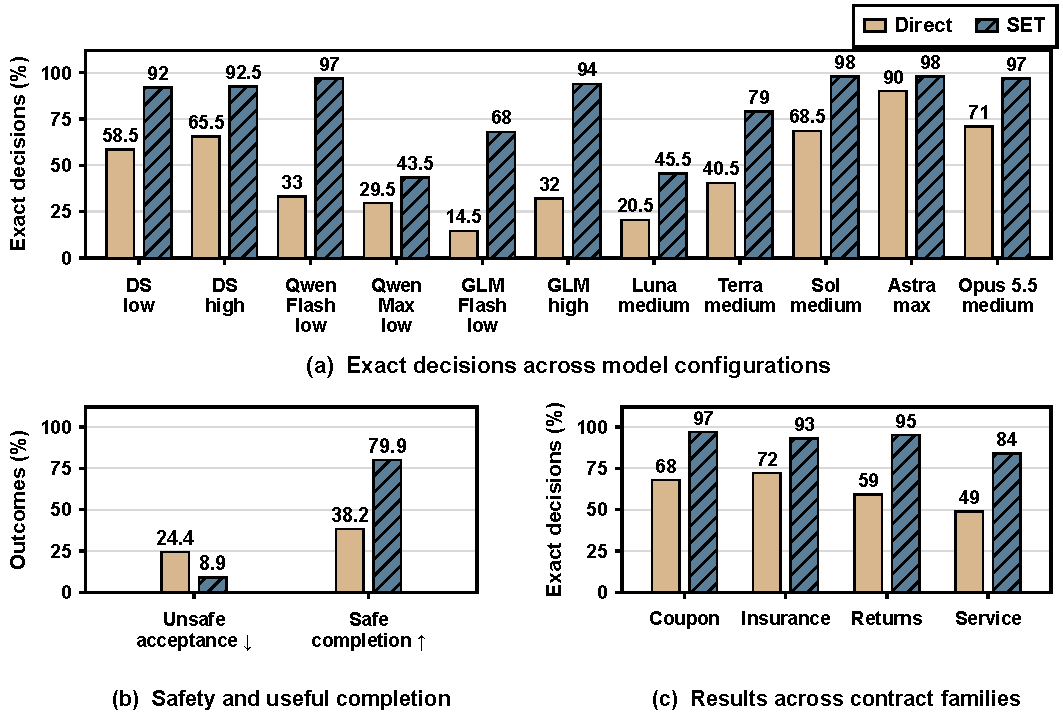
\includegraphics[width=\textwidth]{14_safe_completion.pdf}
\caption{\textbf{Risk-aware decisions across models and contract structures.} Plain bars denote Direct; hatched bars denote SET. (a) Exact-decision rates by configuration (DS: DeepSeek). (b) All eleven configurations: unsafe acceptance over 2,200 outcomes and safe completion over 1,100 feasible outcomes per method. (c) DeepSeek low/high across four contract families, each pooling 100 outcomes per method from five templates. Axes start at zero; configurations share tasks.}
\label{fig:completion}
\end{figure*}

\begin{figure}[!t]
\centering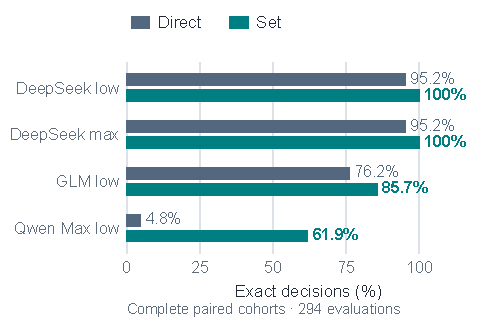
\includegraphics[width=\columnwidth]{16_retained_intent.pdf}
\caption{\textbf{Decisions with unresolved user intent.} Exact-decision rates over 294 outcomes from 147 matched task--configuration pairs, using each configuration's denominator. Compilation is catalogue-visible and ambiguity is explicitly signaled. Appendix~\ref{app:intent} gives counts and errors.}
\label{fig:intent}
\end{figure}

\subsection{Useful Completion at Authorization Boundaries}
\label{sec:boundaries}
All eleven primary configurations improve exactness and safe completion while reducing unsafe acceptances and false refusals (Figure~\ref{fig:completion}). For DeepSeek low/high, exact decisions rise from 248/400 (62.0\%) to 369/400 (92.25\%). The gain is 30.25 percentage points, with a 95\% template-cluster bootstrap interval of $[22.75,37.25]$, retaining both settings within each template. Exact purchases rise from 100 to 186 across 200 feasible outcomes; unsafe acceptances fall from 79 to 9 and false refusals from 53 to 1. On these tasks, stronger safety accompanies more useful purchases and fewer missed opportunities.

Gains cover all four contract families and 18 of 20 templates at each DeepSeek setting. They vary across models: GLM high improves from 64/200 to 188/200, Sol medium from 137/200 to 196/200, and Opus medium from 142/200 to 194/200. Qwen Max low rises from 59 to 87 exact outcomes but retains 46 unsafe acceptances. Appendix~\ref{app:statistics} gives complete partitions and template results. These pairs test authorization boundaries; their unique feasible offers limit conclusions about ranking.

\subsection{Purchasing under Signaled Intent Ambiguity}
\label{sec:intent-decisions}
Figure~\ref{fig:intent} reports 294 outcomes from 147 matched task--configuration pairs covering ticket-holder reference, conditional hotel cancellation, and individual versus batch exchange-cost limits. Both methods receive the catalogue, ambiguity cues, and decision policy; SET's primary compilation instead withholds catalogues. Table~\ref{tab:intent-figure3} gives denominators.

SET improves exactness in all four configurations as risk limits, penalties, and the positive-value boundary vary. Qwen records six unsafe acceptances with SET and five with Direct, so better exactness does not ensure fewer unsafe actions in every panel. Separate checks illustrate common purchases, empty intersections, worst-case ranking, and the zero-value boundary (Appendix~\ref{app:intent-boundaries}); they do not establish a comparative accuracy advantage.

\paragraph{Checks on the workflow comparison.}
\label{sec:robustness}
On the 60-task reasoning panel, SET improves exactness in 17 of 18 Sol/Terra/Luna settings; Luna off falls from 25/60 to 13/60. Across six DeepSeek setting--language cells, Direct achieves 33--36/60 exact decisions and SET 55--59/60. Appendix~\ref{app:execution} gives these panels (Figure~\ref{fig:robustness}), textual-guidance and output-budget controls, and their scope. These checks assess the observed workflow gains, but do not establish that every permission encoded by a successful specification is correct. We next freeze the specification to examine that stronger requirement.

\subsection{Authorization beyond the Selected Purchase}
\label{sec:permissions}
\label{sec:components}
\paragraph{Frozen-specification test.}
We freeze 800 new requests from 20 templates in four contract families, each with 128 offers. Evaluating them under three configurations yields 2,400 planned request--configuration units. DeepSeek Flash, GLM, and Qwen Max, all at low effort, receive requests, contracts, and schemas without catalogues. Catalogues are fixed before generation and stratified by whether their highest-reference-value offer is authorized. The same request and catalogue are shared across configurations; distinct numerical instances do not constitute distinct logical structures. Appendix~\ref{app:availability} gives construction and output-retention rules.

The primary stress test removes prefixes of the original generated ranking, without using reference labels to choose removals. Exposure requires an initially safe purchase to become unauthorized within eight removals, while an alternative remains permitted and positively valued under both generated conditions and references. This predeclared budget removes at most 6.25\% of the 128 offers; curves also report budgets of one, four, and sixteen. Permissions, utilities, surviving attributes, and the selector stay fixed; replays make no model calls. Each unit contributes at most one exposure per budget, irrespective of how many reduced catalogues trigger it.

\begin{figure}[!t]
\centering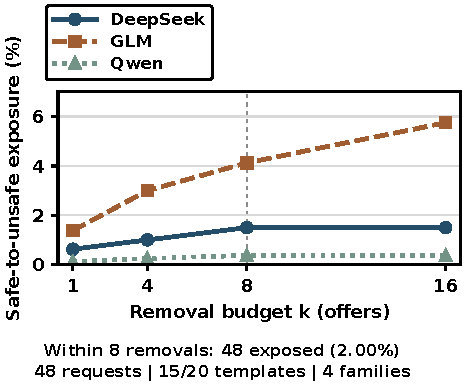
\includegraphics[width=\columnwidth]{13_authorization_diagnostics.pdf}
\caption{\textbf{Availability exposes permission errors despite viable alternatives.} Percentages use 800 planned request--configuration units per model and 2,400 overall. Exposure is cumulative within $k$ removals along the original generated ranking, with a jointly authorized, positive-value alternative retained. The primary budget is $k=8$. These directed tests do not estimate random-stockout probability. Appendix~\ref{app:availability-results} gives conditional counts, coverage, and controls.}
\label{fig:ablations}
\end{figure}

\paragraph{Hidden permissions and behavioral exposure.}
Across the planned cohort, 71 specifications (\AvailHiddenPct\%) produce safe purchases that conceal false admissions. Forty-eight meet the primary exposure endpoint, corresponding to \AvailExposedRequests{} distinct request inputs and \AvailExposedPct\% of planned units. Figure~\ref{fig:ablations} shows cumulative exposure by removal budget. The witnesses cover \AvailExposedTemplates{} templates, all four families, and all three configurations. At each specification's first exposing prefix, \AvailBackupMin{}--\AvailBackupMax{} viable authorized alternatives remain. Every exposed maximizer is unauthorized, so these transitions do not depend on mixed-authorization ties. Native-expression replay and independent contract calculations verify the witnesses.

The controls delimit this result. All primary exposures occur in S, where an authorized offer has the highest reference value. This stratum creates opportunities for masking but does not determine the permissions or utilities the model generates. The random-removal control at $k=8$ gives 0.035\% mean exposure over planned units. It averages 32 draws per unit, whereas the directed endpoint asks whether any tested prefix exposes an error; the two percentages describe different events. Sixty-one of the 71 hidden-error specifications are exposed within sixteen ranked removals. The remaining cases, zero-event templates, and reverse transitions are retained in Appendix~\ref{app:availability-results}. These observations characterize the controlled setting, without establishing a typical market failure rate.

\paragraph{Exposure from exact decisions.}
Eight exposed specifications initially select a reference maximizer and report its value correctly, spanning four templates and two configurations. In one GLM coupon-cancellation case, removing four high-ranked offers makes the frozen specification select an unauthorized purchase while 59 viable authorized alternatives remain. The specification omits a contractual charge when evaluating the newly selected offer, underestimating its loss and admitting it despite a reference loss above the authorized cap. Its original answer was correct; its permission for the alternative was not. Appendix~\ref{app:availability-witness} traces the charge through the expression and event ledger.

\paragraph{From intent to executable decisions.}
Candidate removal changes which admitted offer wins, not whether a surviving offer is authorized. The remaining viable alternatives are also permitted and positively valued by the specification itself. Thus the observed failure requires neither a new model response nor the loss of all useful authorized choices. The error lies in a permission already carried from the request into the executable conditions. The original purchase did not exercise that permission; the changed catalogue does.

These results motivate three separate evaluation outputs when reference semantics are available: current-decision correctness, catalogue-wide false admissions and exclusions, and behavioral exposure under specified availability changes. The first measures useful completion, the second checks fidelity beyond the selected purchase, and the third connects a domain error to an observable action. A replay certificate identifies the unchanged specification, removed offers, unauthorized winner, and surviving viable alternatives. Such certificates provide controlled counterexamples. Passing a bounded availability test does not certify the admitted domain, and evaluating that domain cannot replace the value and completion checks needed for useful delegation.

\section{Conclusion}
Risk-aware delegation must preserve authorization from intent to decision. SET makes generated permissions inspectable and improves useful decisions across the tested configurations. Our frozen-specification tests nevertheless expose false admissions under changed availability, even while viable authorized alternatives remain. Cross-template results and original-expression checks connect these purchases to existing permission errors. Where reference semantics are available, evaluation should distinguish current-decision correctness, domain errors, and their behavioral exposure. Passing a bounded availability test cannot certify the admitted domain. A delegated agent may choose a different offer; doing so must still respect the same authorization.
\label{mainend}

\section*{Limitations}
The evaluated contracts are synthetic, with complete catalogues, known attributes, correct item grounding, and finite state sets. Risk limits and utility are supplied as inputs. The main benchmark isolates authorization boundaries. Its unique feasible candidate provides limited evidence about ranking among several admissible purchases. The availability study instead retains multiple viable purchases and tests a constructed, reference-stratified distribution. Its directed-removal rates describe pressure on frozen specifications, not random stockouts or deployment frequencies. Intent tests signal unresolved readings explicitly. The evaluation does not cover open-ended interpretation discovery, hidden merchant terms, unknown inventory, fraud, or settlement.

Decision conditions can omit a relevant requirement or bind it to the wrong state, even when the resulting specification executes successfully. Reference implementations check consistency with stipulated semantics and share a development workflow. Configuration, language, and diagnostic panels overlap and do not provide independent task samples. Catalogue visibility and provider compute differ across some controls. The appendix specifies the reported cohorts and evaluation protocols. Workflow gains concern the complete decision process; availability replays test frozen generated conditions. Earlier selected-output and exploratory studies remain separately archived and are not pooled with these results.

\section*{Ethical Considerations}
All purchases are synthetic, with no monetary transfers or customer records. Financial consequences follow stipulated benchmark contracts. Saved artifacts distinguish original responses, reference-assisted interventions, and subsequent analysis. In deployment, erroneous acceptance could cause financial loss, while erroneous refusal could prevent access to a needed service. A deployed system would need explicit authorization and failure handling. Correct execution alone cannot establish that a compiled specification faithfully represents the user's request.

\begin{thebibliography}{46}
\providecommand{\natexlab}[1]{#1}

\bibitem[{Andriushchenko et~al.(2025)Andriushchenko, Souly, Dziemian, Duenas, Lin, Wang, Hendrycks, Zou, Kolter, Fredrikson, Gal, and Davies}]{agentharm}
Maksym Andriushchenko, Alexandra Souly, Mateusz Dziemian, Derek Duenas, Maxwell Lin, Justin Wang, Dan Hendrycks, Andy Zou, Zico Kolter, Matt Fredrikson, Yarin Gal, and Xander Davies. 2025.
\newblock \href {https://proceedings.iclr.cc/paper_files/paper/2025/hash/c493d23af93118975cdbc32cbe7323f5-Abstract-Conference.html} {{AgentHarm}: A benchmark for measuring harmfulness of {LLM} agents}.
\newblock In \emph{The Thirteenth International Conference on Learning Representations}, pages 79185--79220.

\bibitem[{Angelopoulos et~al.(2024)Angelopoulos, Bates, Fisch, Lei, and Schuster}]{crc}
Anastasios~N. Angelopoulos, Stephen Bates, Adam Fisch, Lihua Lei, and Tal Schuster. 2024.
\newblock \href {https://proceedings.iclr.cc/paper_files/paper/2024/file/f3549ef9b5ff520a7e41ff3cc306ab2b-Paper-Conference.pdf} {Conformal risk control}.
\newblock In \emph{International Conference on Learning Representations}, volume 2024, pages 55198--55218.

\bibitem[{Campagna et~al.(2019)Campagna, Xu, Moradshahi, Socher, and Lam}]{campagna2019genie}
Giovanni Campagna, Silei Xu, Mehrad Moradshahi, Richard Socher, and Monica~S. Lam. 2019.
\newblock \href {https://doi.org/10.1145/3314221.3314594} {{Genie}: A generator of natural language semantic parsers for virtual assistant commands}.
\newblock In \emph{Proceedings of the 40th ACM SIGPLAN Conference on Programming Language Design and Implementation}, pages 394--410. Association for Computing Machinery.

\bibitem[{Debenedetti et~al.(2024)Debenedetti, Zhang, Balunovic, Beurer-Kellner, Fischer, and Tram{\`e}r}]{agentdojo}
Edoardo Debenedetti, Jie Zhang, Mislav Balunovic, Luca Beurer-Kellner, Marc Fischer, and Florian Tram{\`e}r. 2024.
\newblock \href {https://doi.org/10.52202/079017-2636} {{AgentDojo}: A dynamic environment to evaluate prompt injection attacks and defenses for {LLM} agents}.
\newblock In \emph{Advances in Neural Information Processing Systems}, volume~37, pages 82895--82920.

\bibitem[{Deng et~al.(2023)Deng, Gu, Zheng, Chen, Stevens, Wang, Sun, and Su}]{deng2023mind2web}
Xiang Deng, Yu~Gu, Boyuan Zheng, Shijie Chen, Samuel Stevens, Boshi Wang, Huan Sun, and Yu~Su. 2023.
\newblock \href {https://doi.org/10.52202/075280-1220} {{Mind2Web}: Towards a generalist agent for the web}.
\newblock In \emph{Advances in Neural Information Processing Systems}, volume~36, pages 28091--28114.

\bibitem[{Dong et~al.(2026)Dong, Hu, Hui, Zhang, Vuli{\'c}, Bobu, and Collier}]{voi}
Yijiang~River Dong, Tiancheng Hu, Zheng Hui, Caiqi Zhang, Ivan Vuli{\'c}, Andreea Bobu, and Nigel Collier. 2026.
\newblock \href {https://doi.org/10.18653/v1/2026.acl-long.1987} {Value of information: A framework for human{--}agent communication}.
\newblock In \emph{Proceedings of the 64th Annual Meeting of the {A}ssociation for {C}omputational {L}inguistics (Volume 1: Long Papers)}, pages 42879--42896, San Diego, California, United States. Association for Computational Linguistics.

\bibitem[{Dror et~al.(2018)Dror, Baumer, Shlomov, and Reichart}]{stats}
Rotem Dror, Gili Baumer, Segev Shlomov, and Roi Reichart. 2018.
\newblock \href {https://doi.org/10.18653/v1/P18-1128} {The hitchhiker{'}s guide to testing statistical significance in natural language processing}.
\newblock In \emph{Proceedings of the 56th Annual Meeting of the Association for Computational Linguistics (Volume 1: Long Papers)}, pages 1383--1392, Melbourne, Australia. Association for Computational Linguistics.

\bibitem[{Gao et~al.(2023)Gao, Madaan, Zhou, Alon, Liu, Yang, Callan, and Neubig}]{pal}
Luyu Gao, Aman Madaan, Shuyan Zhou, Uri Alon, Pengfei Liu, Yiming Yang, Jamie Callan, and Graham Neubig. 2023.
\newblock \href {https://proceedings.mlr.press/v202/gao23f.html} {{PAL}: Program-aided language models}.
\newblock In \emph{Proceedings of the 40th International Conference on Machine Learning}, volume 202 of \emph{Proceedings of Machine Learning Research}, pages 10764--10799. PMLR.

\bibitem[{Gardner et~al.(2020)Gardner, Artzi, Basmova, Berant, Bogin, Chen, Dasigi, Dua, Elazar, Gottumukkala, Gupta, Hajishirzi, Ilharco, Khashabi, Lin, Liu, Liu, Mulcaire, Ning, Singh, Smith, Subramanian, Tsarfaty, Wallace, Zhang, and Zhou}]{contrastsets}
Matt Gardner, Yoav Artzi, Victoria Basmova, Jonathan Berant, Ben Bogin, Sihao Chen, Pradeep Dasigi, Dheeru Dua, Yanai Elazar, Ananth Gottumukkala, Nitish Gupta, Hanna Hajishirzi, Gabriel Ilharco, Daniel Khashabi, Kevin Lin, Jiangming Liu, Nelson~F. Liu, Phoebe Mulcaire, Qiang Ning, and 7 others. 2020.
\newblock \href {https://doi.org/10.18653/v1/2020.findings-emnlp.117} {Evaluating models' local decision boundaries via contrast sets}.
\newblock In \emph{Findings of the Association for Computational Linguistics: EMNLP 2020}, pages 1307--1323, Online. Association for Computational Linguistics.

\bibitem[{Gupta et~al.(2018)Gupta, Shah, Mohit, Kumar, and Lewis}]{gupta2018hierarchical}
Sonal Gupta, Rushin Shah, Mrinal Mohit, Anuj Kumar, and Michael Lewis. 2018.
\newblock \href {https://doi.org/10.18653/v1/D18-1300} {Semantic parsing for task oriented dialog using hierarchical representations}.
\newblock In \emph{Proceedings of the 2018 Conference on Empirical Methods in Natural Language Processing}, pages 2787--2792. Association for Computational Linguistics.

\bibitem[{Ivanova et~al.(2025)Ivanova, Bakaeva, Volovikova, Kovalev, and Panov}]{ambik}
Anastasiia Ivanova, Eva Bakaeva, Zoya Volovikova, Alexey~K. Kovalev, and Aleksandr~I. Panov. 2025.
\newblock \href {https://doi.org/10.18653/v1/2025.acl-long.1593} {{A}mbi{K}: Dataset of ambiguous tasks in kitchen environment}.
\newblock In \emph{Proceedings of the 63rd Annual Meeting of the Association for Computational Linguistics (Volume 1: Long Papers)}, pages 33216--33241, Vienna, Austria. Association for Computational Linguistics.

\bibitem[{Kiyani et~al.(2025)Kiyani, Pappas, Roth, and Hassani}]{rac}
Shayan Kiyani, George~J. Pappas, Aaron Roth, and Hamed Hassani. 2025.
\newblock \href {https://proceedings.mlr.press/v267/kiyani25a.html} {Decision theoretic foundations for conformal prediction: Optimal uncertainty quantification for risk-averse agents}.
\newblock In \emph{Proceedings of the 42nd International Conference on Machine Learning}, volume 267 of \emph{Proceedings of Machine Learning Research}, pages 30943--30965. PMLR.

\bibitem[{Levy et~al.(2026)Levy, Wiesel, Marreed, Oved, Yaeli, Mashkif, and Shlomov}]{stwebagentbench}
Ido Levy, Ben Wiesel, Sami Marreed, Alon Oved, Avi Yaeli, Nir Mashkif, and Segev Shlomov. 2026.
\newblock \href {https://proceedings.iclr.cc/paper_files/paper/2026/hash/c6c29e590e3c62e37e6b39cdd6baf2e8-Abstract-Conference.html} {{ST-WebAgentBench}: A benchmark for evaluating safety and trustworthiness in web agents}.
\newblock In \emph{International Conference on Learning Representations}, pages 122213--122255.

\bibitem[{Liu et~al.(2023)Liu, Wu, Michael, Suhr, West, Koller, Swayamdipta, Smith, and Choi}]{liu2023ambiguity}
Alisa Liu, Zhaofeng Wu, Julian Michael, Alane Suhr, Peter West, Alexander Koller, Swabha Swayamdipta, Noah~A. Smith, and Yejin Choi. 2023.
\newblock \href {https://doi.org/10.18653/v1/2023.emnlp-main.51} {We're afraid language models aren't modeling ambiguity}.
\newblock In \emph{Proceedings of the 2023 Conference on Empirical Methods in Natural Language Processing}, pages 790--807. Association for Computational Linguistics.

\bibitem[{Liu et~al.(2026)Liu, Wang, Huang, Li, Li, Guo, Fan, Sarikaya, and Ji}]{complexpolicy}
Jiateng Liu, Zhenhailong Wang, Xiaojiang Huang, Yingjie Li, Xiang Li, Chenlei Guo, Xing Fan, Ruhi Sarikaya, and Heng Ji. 2026.
\newblock \href {https://doi.org/10.18653/v1/2026.acl-long.767} {Analyzing and internalizing complex policy documents for {LLM} agents}.
\newblock In \emph{Proceedings of the 64th Annual Meeting of the Association for Computational Linguistics (Volume 1: Long Papers)}, pages 16814--16851, San Diego, California, United States. Association for Computational Linguistics.

\bibitem[{Liu(2025)}]{folcode}
Junnan Liu. 2025.
\newblock \href {https://doi.org/10.18653/v1/2025.naacl-long.547} {Few-shot natural language to first-order logic translation via code generation}.
\newblock In \emph{Proceedings of the 2025 Conference of the Nations of the Americas Chapter of the Association for Computational Linguistics: Human Language Technologies (Volume 1: Long Papers)}, pages 10939--10960, Albuquerque, New Mexico. Association for Computational Linguistics.

\bibitem[{Luo et~al.(2025)Luo, Dai, Ni, Li, Zhang, Wang, Liu, and Salam}]{agentauditor}
Hanjun Luo, Shenyu Dai, Chiming Ni, Xinfeng Li, Guibin Zhang, Kun Wang, Tongliang Liu, and Hanan Salam. 2025.
\newblock \href {https://doi.org/10.52202/085713-1440} {{AgentAuditor}: Human-level safety and security evaluation for {LLM} agents}.
\newblock In \emph{Advances in Neural Information Processing Systems}, volume~38, pages 43241--43298. Curran Associates, Inc.

\bibitem[{McCoy et~al.(2019)McCoy, Pavlick, and Linzen}]{mccoy2019right}
R.~Thomas McCoy, Ellie Pavlick, and Tal Linzen. 2019.
\newblock \href {https://doi.org/10.18653/v1/P19-1334} {Right for the wrong reasons: Diagnosing syntactic heuristics in natural language inference}.
\newblock In \emph{Proceedings of the 57th Annual Meeting of the Association for Computational Linguistics}, pages 3428--3448. Association for Computational Linguistics.

\bibitem[{Miculicich et~al.(2026)Miculicich, Parmar, Palangi, Dvijotham, Montanari, Pfister, and Le}]{veriguard}
Lesly Miculicich, Mihir Parmar, Hamid Palangi, Krishnamurthy~Dj Dvijotham, Mirko Montanari, Tomas Pfister, and Long~T. Le. 2026.
\newblock \href {https://research.google/pubs/veriguard-enhancing-llm-agent-safety-via-verified-code-generation-2/} {{VeriGuard}: Enhancing {LLM} agent safety via verified code generation}.
\newblock In \emph{ACL 2026}.

\bibitem[{Min et~al.(2020)Min, Michael, Hajishirzi, and Zettlemoyer}]{min2020ambigqa}
Sewon Min, Julian Michael, Hannaneh Hajishirzi, and Luke Zettlemoyer. 2020.
\newblock \href {https://doi.org/10.18653/v1/2020.emnlp-main.466} {{AmbigQA}: Answering ambiguous open-domain questions}.
\newblock In \emph{Proceedings of the 2020 Conference on Empirical Methods in Natural Language Processing (EMNLP)}, pages 5783--5797. Association for Computational Linguistics.

\bibitem[{Ning et~al.(2026)Ning, Jones, Zhang, Ye, Ruan, Li, Gupta, and Sun}]{deaction}
Yuting Ning, Jaylen Jones, Zhehao Zhang, Chentao Ye, Weitong Ruan, Junyi Li, Rahul Gupta, and Huan Sun. 2026.
\newblock \href {https://proceedings.mlr.press/v306/ning26c.html} {When actions go off-task: Detecting and correcting misaligned actions in computer-use agents}.
\newblock In \emph{Proceedings of the 43rd International Conference on Machine Learning}, volume 306 of \emph{Proceedings of Machine Learning Research}, pages 93346--93375. PMLR.

\bibitem[{Olausson et~al.(2023)Olausson, Gu, Lipkin, Zhang, Solar-Lezama, Tenenbaum, and Levy}]{linc}
Theo~X. Olausson, Alex Gu, Benjamin Lipkin, Cedegao~E. Zhang, Armando Solar-Lezama, Joshua~B. Tenenbaum, and Roger Levy. 2023.
\newblock \href {https://doi.org/10.18653/v1/2023.emnlp-main.313} {{LINC}: A neurosymbolic approach for logical reasoning by combining language models with first-order logic provers}.
\newblock In \emph{Proceedings of the 2023 Conference on Empirical Methods in Natural Language Processing}, pages 5153--5176, Singapore. Association for Computational Linguistics.

\bibitem[{Pan et~al.(2023)Pan, Albalak, Wang, and Wang}]{logiclm}
Liangming Pan, Alon Albalak, Xinyi Wang, and William~Yang Wang. 2023.
\newblock \href {https://doi.org/10.18653/v1/2023.findings-emnlp.248} {Logic-{LM}: Empowering large language models with symbolic solvers for faithful logical reasoning}.
\newblock In \emph{Findings of the Association for Computational Linguistics: EMNLP 2023}, pages 3806--3824, Singapore. Association for Computational Linguistics.

\bibitem[{Parikh and Surapaneni(2025)}]{ap2}
Stavan Parikh and Rao Surapaneni. 2025.
\newblock \href {https://cloud.google.com/blog/products/ai-machine-learning/announcing-agents-to-payments-ap2-protocol} {Powering {AI} commerce with the new {Agent Payments Protocol (AP2)}}.
\newblock Google Cloud Blog.

\bibitem[{Pei et~al.(2025)Pei, Du, and Jin}]{fover}
Yu~Pei, Yongping Du, and Xingnan Jin. 2025.
\newblock \href {https://doi.org/10.1162/tacl.a.41} {{F}o{V}er: First-order logic verification for natural language reasoning}.
\newblock \emph{Transactions of the Association for Computational Linguistics}, 13:1340--1359.

\bibitem[{{Peyton Jones} et~al.(2000){Peyton Jones}, Eber, and Seward}]{composingcontracts}
Simon {Peyton Jones}, Jean-Marc Eber, and Julian Seward. 2000.
\newblock \href {https://www.microsoft.com/en-us/research/publication/composing-contracts-an-adventure-in-financial-engineering/} {Composing contracts: An adventure in financial engineering}.
\newblock In \emph{Proceedings of the ACM SIGPLAN International Conference on Functional Programming}, pages 280--292. ACM.

\bibitem[{Qi et~al.(2025)Qi, Peng, Wang, Xin, Liu, Xu, Hou, and Li}]{agentif}
Yunjia Qi, Hao Peng, Xiaozhi Wang, Amy Xin, Youfeng Liu, Bin Xu, Lei Hou, and Juanzi Li. 2025.
\newblock \href {https://doi.org/10.52202/085713-1892} {{AgentIF}: Benchmarking instruction following of large language models in agentic scenarios}.
\newblock In \emph{Advances in Neural Information Processing Systems}, volume~38. Curran Associates, Inc.
\newblock Datasets and Benchmarks Track.

\bibitem[{Quansah et~al.(2026)Quansah, Rivas~Perea, and Bonnah}]{verify}
Paapa~Kwesi Quansah, Pablo Rivas~Perea, and Ernest Bonnah. 2026.
\newblock \href {https://proceedings.iclr.cc/paper_files/paper/2026/file/8b078da44614b6e249dc9e9474dc8d11-Paper-Conference.pdf} {{VERIFY}: A novel multi-domain dataset grounding {LTL} in contextual natural language via provable intermediate logic}.
\newblock In \emph{International Conference on Learning Representations}, volume 2026, pages 86416--86453.

\bibitem[{Rabinovich et~al.(2026)Rabinovich, Boaz, Zwerdling, and Anaby-Tavor}]{nearmiss}
Ella Rabinovich, David Boaz, Naama Zwerdling, and Ateret Anaby-Tavor. 2026.
\newblock \href {https://doi.org/10.18653/v1/2026.gem-main.30} {{Near-Miss}: Latent policy failure detection in agentic workflows}.
\newblock In \emph{Proceedings of the Fifth Workshop on Generation, Evaluation and Metrics ({GEM})}, pages 296--308, San Diego, California, USA. Association for Computational Linguistics.

\bibitem[{Ren et~al.(2023)Ren, Dixit, Bodrova, Singh, Tu, Brown, Xu, Takayama, Xia, Varley, Xu, Sadigh, Zeng, and Majumdar}]{knowno}
Allen~Z. Ren, Anushri Dixit, Alexandra Bodrova, Sumeet Singh, Stephen Tu, Noah Brown, Peng Xu, Leila Takayama, Fei Xia, Jake Varley, Zhenjia Xu, Dorsa Sadigh, Andy Zeng, and Anirudha Majumdar. 2023.
\newblock \href {https://proceedings.mlr.press/v229/ren23a.html} {Robots that ask for help: Uncertainty alignment for large language model planners}.
\newblock In \emph{Proceedings of The 7th Conference on Robot Learning}, volume 229 of \emph{Proceedings of Machine Learning Research}, pages 661--682. PMLR.

\bibitem[{Ribeiro et~al.(2020)Ribeiro, Wu, Guestrin, and Singh}]{checklist}
Marco~Tulio Ribeiro, Tongshuang Wu, Carlos Guestrin, and Sameer Singh. 2020.
\newblock \href {https://doi.org/10.18653/v1/2020.acl-main.442} {Beyond accuracy: Behavioral testing of {NLP} models with {C}heck{L}ist}.
\newblock In \emph{Proceedings of the 58th Annual Meeting of the Association for Computational Linguistics}, pages 4902--4912, Online. Association for Computational Linguistics.

\bibitem[{Ruan et~al.(2024)Ruan, Dong, Wang, Pitis, Zhou, Ba, Dubois, Maddison, and Hashimoto}]{toolemu}
Yangjun Ruan, Honghua Dong, Andrew Wang, Silviu Pitis, Yongchao Zhou, Jimmy Ba, Yann Dubois, Chris~J. Maddison, and Tatsunori Hashimoto. 2024.
\newblock \href {https://proceedings.iclr.cc/paper_files/paper/2024/hash/7274ed909a312d4d869cc328ad1c5f04-Abstract-Conference.html} {Identifying the risks of {LM} agents with an {LM}-emulated sandbox}.
\newblock In \emph{The Twelfth International Conference on Learning Representations}, pages 27031--27098.

\bibitem[{Schick et~al.(2023)Schick, Dwivedi-Yu, Dess{\`i}, Raileanu, Lomeli, Hambro, Zettlemoyer, Cancedda, and Scialom}]{schick2023toolformer}
Timo Schick, Jane Dwivedi-Yu, Roberto Dess{\`i}, Roberta Raileanu, Maria Lomeli, Eric Hambro, Luke Zettlemoyer, Nicola Cancedda, and Thomas Scialom. 2023.
\newblock \href {https://doi.org/10.52202/075280-2997} {{Toolformer}: Language models can teach themselves to use tools}.
\newblock In \emph{Advances in Neural Information Processing Systems}, volume~36, pages 68539--68551.

\bibitem[{Shin et~al.(2021)Shin, Lin, Thomson, Chen, Roy, Platanios, Pauls, Klein, Eisner, and {Van Durme}}]{shin2021constrained}
Richard Shin, Christopher~H. Lin, Sam Thomson, Charles Chen, Subhro Roy, Emmanouil~Antonios Platanios, Adam Pauls, Dan Klein, Jason Eisner, and Benjamin {Van Durme}. 2021.
\newblock \href {https://doi.org/10.18653/v1/2021.emnlp-main.608} {Constrained language models yield few-shot semantic parsers}.
\newblock In \emph{Proceedings of the 2021 Conference on Empirical Methods in Natural Language Processing}, pages 7699--7715. Association for Computational Linguistics.

\bibitem[{Suri et~al.(2026)Suri, Mathur, Lipka, Dernoncourt, Rossi, and Manocha}]{sage}
Manan Suri, Puneet Mathur, Nedim Lipka, Franck Dernoncourt, Ryan~A. Rossi, and Dinesh Manocha. 2026.
\newblock \href {https://doi.org/10.18653/v1/2026.findings-acl.2028} {Structured uncertainty guided clarification for {LLM} agents}.
\newblock In \emph{Findings of the {A}ssociation for {C}omputational {L}inguistics: {ACL} 2026}, pages 40811--40838, San Diego, California, United States. Association for Computational Linguistics.

\bibitem[{Vijayvargiya et~al.(2026)Vijayvargiya, Soni, Zhou, Wang, Dziri, Neubig, and Sap}]{openagentsafety}
Sanidhya Vijayvargiya, Aditya~Bharat Soni, Xuhui Zhou, Zora~Zhiruo Wang, Nouha Dziri, Graham Neubig, and Maarten Sap. 2026.
\newblock \href {https://proceedings.iclr.cc/paper_files/paper/2026/hash/a0f6c06b8d6114bb37688c2dc19b4d74-Abstract-Conference.html} {{OpenAgentSafety}: A comprehensive framework for evaluating real-world {AI} agent safety}.
\newblock In \emph{International Conference on Learning Representations}, pages 99089--99114.

\bibitem[{Wang et~al.(2026)Wang, Poskitt, and Sun}]{agentspec}
Haoyu Wang, Christopher~M. Poskitt, and Jun Sun. 2026.
\newblock \href {https://doi.org/10.1145/3744916.3764546} {{AgentSpec}: Customizable runtime enforcement for safe and reliable {LLM} agents}.
\newblock In \emph{Proceedings of the 48th IEEE/ACM International Conference on Software Engineering}, pages 2938--2950.

\bibitem[{Xiang et~al.(2025)Xiang, Zheng, Li, Hong, Li, Xie, Zhang, Xiong, Xie, Yang, Song, and Li}]{guardagent}
Zhen Xiang, Linzhi Zheng, Yanjie Li, Junyuan Hong, Qinbin Li, Han Xie, Jiawei Zhang, Zidi Xiong, Chulin Xie, Carl Yang, Dawn Song, and Bo~Li. 2025.
\newblock \href {https://proceedings.mlr.press/v267/xiang25a.html} {{G}uard{A}gent: Safeguard {LLM} agents via knowledge-enabled reasoning}.
\newblock In \emph{Proceedings of the 42nd International Conference on Machine Learning}, volume 267 of \emph{Proceedings of Machine Learning Research}, pages 68316--68342. PMLR.

\bibitem[{Xie et~al.(2024)Xie, Zhang, Chen, Zhu, Lou, Tian, Xiao, and Su}]{travelplanner}
Jian Xie, Kai Zhang, Jiangjie Chen, Tinghui Zhu, Renze Lou, Yuandong Tian, Yanghua Xiao, and Yu~Su. 2024.
\newblock \href {https://proceedings.mlr.press/v235/xie24j.html} {{T}ravel{P}lanner: A benchmark for real-world planning with language agents}.
\newblock In \emph{Proceedings of the 41st International Conference on Machine Learning}, volume 235 of \emph{Proceedings of Machine Learning Research}, pages 54590--54613. PMLR.

\bibitem[{Yao et~al.(2022)Yao, Chen, Yang, and Narasimhan}]{webshop}
Shunyu Yao, Howard Chen, John Yang, and Karthik Narasimhan. 2022.
\newblock \href {https://doi.org/10.52202/068431-1508} {{WebShop}: Towards scalable real-world web interaction with grounded language agents}.
\newblock In \emph{Advances in Neural Information Processing Systems}, volume~35, pages 20744--20757. Curran Associates, Inc.

\bibitem[{Yao et~al.(2025)Yao, Shinn, Razavi, and Narasimhan}]{taubench}
Shunyu Yao, Noah Shinn, Pedram Razavi, and Karthik Narasimhan. 2025.
\newblock \href {https://proceedings.iclr.cc/paper_files/paper/2025/hash/1b126cc38b8638e07bef37e7b2bb72bf-Abstract-Conference.html} {{$\tau$}-bench: A benchmark for tool-agent-user interaction in real-world domains}.
\newblock In \emph{The Thirteenth International Conference on Learning Representations}, pages 9965--10017.

\bibitem[{Yao et~al.(2023)Yao, Zhao, Yu, Du, Shafran, Narasimhan, and Cao}]{react}
Shunyu Yao, Jeffrey Zhao, Dian Yu, Nan Du, Izhak Shafran, Karthik Narasimhan, and Yuan Cao. 2023.
\newblock \href {https://react-lm.github.io/} {{ReAct}: Synergizing reasoning and acting in language models}.
\newblock In \emph{International Conference on Learning Representations (ICLR)}.

\bibitem[{Ye et~al.(2024)Ye, Li, Li, Huang, Gao, Wu, Zhang, Gui, and Huang}]{ye2024toolsword}
Junjie Ye, Sixian Li, Guanyu Li, Caishuang Huang, Songyang Gao, Yilong Wu, Qi~Zhang, Tao Gui, and Xuanjing Huang. 2024.
\newblock \href {https://doi.org/10.18653/v1/2024.acl-long.119} {{ToolSword}: Unveiling safety issues of large language models in tool learning across three stages}.
\newblock In \emph{Proceedings of the 62nd Annual Meeting of the Association for Computational Linguistics (Volume 1: Long Papers)}, pages 2181--2211. Association for Computational Linguistics.

\bibitem[{Zhang and Choi(2025)}]{intentsim}
Michael~J.Q. Zhang and Eunsol Choi. 2025.
\newblock \href {https://doi.org/10.18653/v1/2025.findings-naacl.306} {Clarify when necessary: Resolving ambiguity through interaction with {LM}s}.
\newblock In \emph{Findings of the Association for Computational Linguistics: NAACL 2025}, pages 5541--5558, Albuquerque, New Mexico. Association for Computational Linguistics.

\bibitem[{Zhou et~al.(2024)Zhou, Xu, Zhu, Zhou, Lo, Sridhar, Cheng, Ou, Bisk, Fried, Alon, and Neubig}]{zhou2024webarena}
Shuyan Zhou, Frank~F. Xu, Hao Zhu, Xuhui Zhou, Robert Lo, Abishek Sridhar, Xianyi Cheng, Tianyue Ou, Yonatan Bisk, Daniel Fried, Uri Alon, and Graham Neubig. 2024.
\newblock \href {https://proceedings.iclr.cc/paper_files/paper/2024/hash/4410c0711e9154a7a2d26f9b3816d1ef-Abstract-Conference.html} {{WebArena}: A realistic web environment for building autonomous agents}.
\newblock In \emph{The Twelfth International Conference on Learning Representations}, pages 15585--15606.

\bibitem[{Zhu et~al.(2026)Zhu, Kiyani, Pappas, and Hassani}]{actionrac}
Zihan Zhu, Shayan Kiyani, George~J. Pappas, and Hamed Hassani. 2026.
\newblock \href {https://proceedings.mlr.press/v306/zhu26z.html} {Conformal risk-averse decision making with action conditional guarantee}.
\newblock In \emph{Proceedings of the 43rd International Conference on Machine Learning}, volume 306 of \emph{Proceedings of Machine Learning Research}, pages 167248--167276. PMLR.

\end{thebibliography}

\clearpage
\appendix
\setcounter{dbltopnumber}{2}
\renewcommand{\dbltopfraction}{0.7}
\makeatletter
\setlength{\@dblfptop}{0pt}
\setlength{\@dblfpsep}{18pt}
\setlength{\@dblfpbot}{0pt plus 1fil}
\makeatother
% Method and evidence supplement; development records remain in the archive.
\noindent\textbf{Appendix guide.} A: decision semantics and implementation; B: tasks and protocol;
C: complete primary results; D: retained-intent decisions;
E: textual guidance and sensitivity; F: availability study and verification.
\section{Decision Semantics and Implementation Details}
\label{app:proofs}
\subsection{Decision semantics and assumptions}
The formulation in Section~\ref{sec:method} fixes a nonempty retained state set and utilities on a common cardinal scale, bounded over the finite experimental domain. It requires no unique reading, state probabilities, linearity, or convexity. Correct execution implies correctness for the request only when generated conditions preserve its decision-relevant semantics. We use RAC's fixed-set principle \citep{rac}, without implementing conformal coverage or action-conditional calibration.

\label{app:ambiguity}

\subsection{Generated conditions and evaluation}
\label{app:interface}
The SET implementation uses a small expression language to encode the conditions used by Algorithm~\ref{alg:decision}. A specification $Q$ contains state-indexed clauses $(\widehat H_j,\widehat R_j,\widehat u_j)$. Each state record contains a label and expressions \texttt{hard}, \texttt{risk}, and \texttt{utility}. Boolean expressions support conjunction, disjunction, negation, comparisons, and conditionals. Arithmetic supports exact literals, basic operations, minimum, maximum, and absolute value. Boolean and numeric values have distinct types. Expression variables refer to attributes in the schema. A missing attribute needed for a feasibility check leaves that check uncertified. The primary benchmark provides complete attributes.

For the $K$ generated clauses, indexed by $j=1,\ldots,K$, evaluation gives
\begin{align}
\widehat f(z)&=\bigwedge_{j=1}^{K}(\widehat H_j(z)\wedge\widehat R_j(z)),\\
\widehat\psi(z)&=\min_{1\le j\le K}\widehat u_j(z).
\end{align}
Algorithm~\ref{alg:decision} requires complete enumeration of $C$, a decided $\widehat f(z)$ for every candidate, and known state utilities whenever $\widehat f(z)=1$. A known false conjunct determines an aggregate predicate even if another conjunct is unknown. Invalid expressions or unresolved required checks produce failure before selection. The evaluator forms $\widehat F_C=\{z\in C:\widehat f(z)=1\}$ and its maximizing set $Z^\star$. The scorer accepts a nonempty subset of tied positive-value maximizers with the correct guaranteed value; one complete purchase is chosen from that subset. Equivalent merged clauses may encode the same decision functions.

\paragraph{Exactness on the declared domain.}
After these checks, membership in $\widehat F_C$ is decided for every $z\in C$, and all values over that domain are known. Finite enumeration therefore returns the complete set of maximizers when the maximum is positive. Otherwise, an empty domain or a nonpositive maximum proves that the compiled problem has no positive-value option. No unresolved candidate is silently excluded from the optimization.

Incomplete or uncertified execution counts as Other in the outcome protocol (Appendix~\ref{app:implementation}).

Exhaustive evaluation costs $O(MKT)$ for $M$ candidates, $K$ generated states, and expression cost $T$. Concrete syntax, serialization, decoding, and runtime bounds are documented with the implementation in the artifact. The evaluation semantics and certification conditions above apply to the generated specification.

\begin{table}[t]
\centering\small
\begin{minipage}{\columnwidth}
\textbf{Contract:} Up to four of six services may cancel. Insurance pays half the gross loss above an order deductible, capped by coverage. The administrative fee is uncovered.\\[3pt]
\textbf{Generated conditions} (equivalent notation, MU): let $G_4$ sum the four largest component losses; $d,c,a,p$ denote deductible, coverage, admin, and price. The worst net loss is $\widehat L$.
\[
\begin{aligned}
\widehat L&=G_4-\min\{c,\max(0,G_4-d)/2\}+a,\\
\widehat H&=[p\le12{,}000],\quad
\widehat R=[\widehat L\le2{,}000],\\
\widehat u&=20{,}000-p-\widehat L.
\end{aligned}
\]
\end{minipage}
\begin{tabular}{@{}lr@{}}
\toprule
Selected offer: price / gross worst loss & 8,568.35 / 880\\
Deductible / payout cap / admin & 149 / 73 / 1,192\\
Worst net loss / guaranteed value & 1,999 / 9,432.65\\
\bottomrule
\end{tabular}
\caption{\textbf{Observed primary compilation.} DeepSeek high generates the clause without seeing the catalogue. Complete-domain execution selects the authorized offer among 256 candidates. The shortened expressions agree with the retained output and all 57-event reference calculations (Appendix~\ref{app:primary-trace}).}
\label{tab:primary-trace}
\end{table}

\subsection{Observed primary contract compilation}
\label{app:primary-trace}
Table~\ref{tab:primary-trace} uses a retained DeepSeek high output for template b2, second stratum, generated without the catalogue. Its clause sums the four largest losses as the total minus the smallest and second-smallest, expressing the latter through pairwise maxima. We abbreviate this as $G_4$ and rename variables. The table converts original integer subunits to MU by dividing by 100.

For this deductible--coinsurance contract with nonnegative component losses, net loss is nondecreasing in gross loss, so its worst nonempty event uses the four largest losses. The empty event has zero loss. One generated clause represents all 57 events with the same aggregate semantics. Offline verification compares the retained expressions with the displayed notation and the reference ledger across 256 candidates and 14,592 candidate--event calculations. The current complete-domain evaluator reproduces the recorded purchase and value. The source package includes the original expressions, candidate attributes, and verification. This check uses the retained output without a new model call.

\subsection{Recorded ambiguity trace}
\label{app:observed-trace}
Table~\ref{tab:observed-trace} uses archived Astra max SET outputs for F02a/F02b (clean context, first sample). Both inputs include the catalogue and stipulated utility $(3000-p)/1000$. The generated clauses preserve both refund readings: the executor refuses F02a and accepts D in F02b with value $1/5$. Display translation and variable renaming preserve the expressions. Original responses and execution records remain in the artifact. This is a method illustration, not evidence of comparative accuracy.

\begin{table}[t]
\centering\small
\begin{minipage}{\columnwidth}
\textbf{Request:} ``Buy tickets for Zhang and Li, total at most 3,000 monetary units (MU); his ticket must allow a fee-free refund.'' The referent remains unspecified.\\[3pt]
\textbf{Generated clauses} (notation shortened): $p$ is the total price; $r_Z$ and $r_L$ indicate fee-free refundability for Zhang and Li, respectively.
\[
\begin{array}{l|ll}
\text{State} & \widehat H & (\widehat R,\widehat u)\\
\hline
\text{Zhang} & p\le3000\ \wedge\ r_Z &(\mathrm{True},(3000-p)/1000)\\
\text{Li} & p\le3000\ \wedge\ r_L &(\mathrm{True},(3000-p)/1000)
\end{array}
\]
\end{minipage}
\begin{tabular}{@{}lrrcc@{}}
\toprule
Order & Price (MU) & Refunds & Jointly allowed & Value\\
\midrule
B & 2,400 & Zhang & No & ---\\
C & 2,400 & Li & No & ---\\
D & 2,800 & Both & Yes & $1/5$\\
\bottomrule
\end{tabular}
\caption{\textbf{Observed request-to-decision trace.} Astra max generates both clauses: the executor selects D, but refuses a catalogue containing only B and C. Utility is stipulated. Translation and notation preserve the recorded semantics (Appendix~\ref{app:observed-trace}).}
\label{tab:observed-trace}
\end{table}

\subsection{How state omission affects permission and value}
\label{app:omission-analysis}
Fix $x$ and write $\Theta=\Theta(x)$. For a nonempty $S\subseteq\Theta$, let $F_S$ and $\psi_S$ denote the intersection in Equation~\eqref{eq:common} and the worst-case utility in Equation~\eqref{eq:robust}, restricted to states in $S$. Retaining only $\Theta'\subseteq\Theta$, with $\Theta'\ne\varnothing$ and all remaining state functions unchanged, gives
\begin{equation}
F_\Theta\subseteq F_{\Theta'},\qquad
\psi_{\Theta'}(z)\ge\psi_\Theta(z).
\label{eq:omission}
\end{equation}
Removing conjuncts cannot shrink the admissible set, and removing terms cannot lower the worst-case value. A single omission can thus weaken authorization and inflate the value used for selection. Both inequalities can be equalities: a redundant state changes neither quantity. The relevant issue is whether its conditions affect the aggregate, not the number of labels emitted. Equivalent merged conditions preserve the decision semantics.

In the hotel tasks, ``his room'' binds one guest to the arrival-dependent cancellation deadline, fee checked against the cap, and utility penalty. Omitting that reading can remove both a permission check and a source of low value. Incorrect binding is a separate error; Equation~\eqref{eq:omission} assumes deletion with all remaining functions fixed. Appendix~\ref{app:intent} gives the task semantics. Clause aggregation and financial-consequence calculations can also be wrong even when all relevant event terms are present. The availability analysis in Section~\ref{sec:analysis} applies to the resulting domain regardless of the error source.
\section{Benchmark Construction and Experimental Protocol}
\label{app:data}
\label{app:protocol}
\subsection{Contract structures and paired boundaries}
The primary dataset contains 20 templates (Table~\ref{tab:templates}), with five feasible/infeasible pairs per template. Each purchase has six components; the retained events are the 57 affected subsets of size at most four, including the empty event. Empty events have zero assessment. A nonempty event incurs one administrative fee, outside insurance or compensation offsets. Public contracts state that no additional hidden clauses apply.

The master construction seed is 39071007, with predetermined template and stratum offsets. The unique authorized positive-value candidate has loss margin $m$: the authorized cap minus its worst loss, in subunits (Table~\ref{tab:strata}). Increasing only its administrative fee by $m+1$ makes the paired task infeasible, with maximum loss of 200,001 subunits against a 200,000-subunit limit. The resulting violation is always one subunit, although the fee increment depends on the feasible margin. Other candidates already exceed the limit by 1--20,000 subunits. Opaque candidate identifiers contain no answer labels, and positions are sampled before attributes are generated. Amounts are reported in MU without changing the stored values.

\begin{table*}[!tbp]
\centering\small
\begin{tabular}{llp{10.4cm}}
\toprule
ID & Family & Distinct contractual structure \\
\midrule
a1 & Coupon cancellation & Overlapping three-person groups; a clawback applies to partial but not full group cancellation.\\
a2 & Coupon cancellation & Different settlement charges for one versus both members of a two-person group.\\
a3 & Coupon cancellation & A cap on group clawbacks plus a conditional order-level clawback.\\
a4 & Coupon cancellation & A rebate offsets group charges only after multiple groups are broken.\\
a5 & Coupon cancellation & Only the largest group clawback is charged, with a specified combination surcharge.\\
\midrule
b1 & Insured cancellation & Item deductibles and item payout limits, followed by an aggregate payout cap.\\
b2 & Insured cancellation & An order-level deductible followed by proportional coinsurance.\\
b3 & Insured cancellation & The number of cancellations changes the aggregate insurance limit.\\
b4 & Insured cancellation & Primary insurance followed by secondary insurance on remaining loss.\\
b5 & Insured cancellation & Payout is triggered by a strict threshold, then calculated from the first unit of loss.\\
\midrule
c1 & Threshold returns & Two product groups have separate retained-value discount clawbacks.\\
c2 & Threshold returns & Fixed shipping parcels; return freight is the largest item fee within each affected parcel.\\
c3 & Threshold returns & Retained purchase value determines a tiered retained discount.\\
c4 & Threshold returns & Separate retained-value and retained-weight thresholds govern two subsidies.\\
c5 & Threshold returns & Restocking fees are capped; sufficiently large returns waive return freight.\\
\midrule
d1 & Service replacement & Item-level compensation limits apply before an order-level cap.\\
d2 & Service replacement & Activating replacement service incurs a fixed fee per affected group.\\
d3 & Service replacement & The number of failures determines the aggregate compensation cap.\\
d4 & Service replacement & Cash compensation combines with explicitly authorized, discounted service credits.\\
d5 & Service replacement & Overlapping group dispatch fees and threshold-triggered additional compensation.\\
\bottomrule
\end{tabular}
\caption{All 20 primary structures. Numerical instances vary within each template; the four families contain 50 cases each. These contracts define synthetic assessment rules and are not claims about actual merchants' terms.}
\label{tab:templates}
\end{table*}

\begin{table}[!htbp]
\centering\small
\begin{tabular}{rrrr}
\toprule
Stratum & Candidates & Margin (subunits) & Cases\\
\midrule
1 & 128 & 1 & 40\\
2 & 256 & 100 & 40\\
3 & 512 & 10,000 & 40\\
4 & 1,024 & 100 & 40\\
5 & 1,024 & 1 & 40\\
\bottomrule
\end{tabular}
\caption{Each stratum includes one pair for every template. Catalogue size, margin, and seed change together; these strata do not isolate their individual causal effects.}
\label{tab:strata}
\end{table}

The design fixes unique feasibility, balanced acceptance/refusal, and complete catalogues. The task balance is not an estimate of real purchasing frequencies.

\subsection{Reference calculations and freezing}
A cash-flow ledger evaluates bitmask events with integer or rational arithmetic, and a separate expression implementation uses the rule engine. Before model evaluation, we compare candidate feasibility, worst loss, guaranteed utility, and final decisions. They agree on all 6,712,320 candidate--event checks. Twenty fresh attribute assignments per template are also checked on all 64 subsets, yielding $20\times20\times64=25{,}600$ checks, plus three hand-calculated threshold witnesses. These references implement the stipulated benchmark contracts. Cross-implementation, fresh-attribute, and hand-worked checks test internal consistency; they do not establish validity for unobserved merchant terms. Both implementations arose within one development workflow and may share a misunderstanding of a clause despite agreeing numerically.

Tasks, references, prompts, and evaluator code are frozen before model evaluation. Public inputs exclude construction seeds, reference matrices, labels, and designated safe identifiers. Candidate visibility follows Table~\ref{tab:visibility}.

\subsection{Common instructions and outcome protocol}
\label{app:implementation}
Table~\ref{tab:evaluation-coverage} is the protocol index. This section defines primary inputs, policy, and scoring; Section~\ref{app:model-configurations} specifies model settings. Appendix~\ref{app:intent} records the catalogue-visible intent variant, Appendix~\ref{app:execution} the sensitivity controls, and Appendix~\ref{app:availability} the frozen-specification interventions. These cohorts retain their own inputs and denominators.

All primary routes receive the same substantive policy, summarized below in English. The frozen model-facing prompts retain their original language and are unchanged by this summary.
\begin{quote}\small
Retain applicable interpretations. Respect current authorization in every retained state. Evaluate hard requirements and the complete risk permission, then maximize the minimum state-dependent utility. Buy only for positive guaranteed value; otherwise refuse. Do not ask the user or change permissions.
\end{quote}
Direct returns a decision, allowed identifiers, and guaranteed utility. SET returns the state-wise expressions of Appendix~\ref{app:interface}. Exactness requires agreement with the reference decision and, for acceptance, a nonempty subset of authorized maximizers and correct value. Disjoint failures are unsafe acceptance, false refusal, and Other (remaining value or invalid-execution failures). SET executions must satisfy the complete-domain checks in Algorithm~\ref{alg:decision}. Failed or unresolved execution counts as Other, including a no-action output whose reference decision is refusal.

\begin{table}[!htbp]
\centering\small
\begin{tabular}{lcc}
\toprule
Property & Direct & SET\\
\midrule
Natural-language records & Yes & Yes\\
Attribute schema & Yes & Yes\\
Catalogue in model input & Yes & No\\
Deterministic row evaluation & No & Yes\\
Exact arithmetic in executor & --- & Yes\\
Observable allowed domain & No & Yes\\
Model calls per primary trial & 1 & 1\\
\bottomrule
\end{tabular}
\caption{Primary method controls. Different catalogue visibility is a declared architectural choice. ``One call'' refers to a logical trial; transport retries are separately retained.}
\label{tab:visibility}
\end{table}

A primary comparison trial allows one semantic attempt. Transport failures may be retried within the recorded limit; formatting, semantic, and output-budget failures end the trial. We save every received response before scoring and count all failures in completed cohorts. Calls not issued remain missing. We reuse an earlier result only when the messages, schema, requested model, effort setting, deadline, output budget, and both task and reference data are unchanged. Sources are selected without using the outcome.

\subsection{Model configurations}
\label{app:model-configurations}
\label{app:qwen}
\label{app:primary-extensions}
Table~\ref{tab:configurations} combines settings for the primary, intent, and prospective availability studies with the retained inventory of 12 requested models and 49 model--effort combinations. The effort panel uses all six settings for Sol, Terra, and Luna; language tests use DeepSeek low/high/max and Astra max. The inventory also includes additional and archived runs; their exact per-study settings remain in the artifact. Paired Direct/SET comparisons share requested generation settings. Primary command-line interface (CLI) calls use fresh contexts with tools and delegation disabled; application programming interface (API) outputs pass the common validator. Requested effort and output caps do not establish equivalent compute across providers.

\begin{table*}[p]
\centering\fontsize{9}{10.5}\selectfont
\setlength{\tabcolsep}{4pt}
\textbf{A. Settings for the main evaluation cohorts}\par\smallskip
\begin{tabular}{@{}>{\raggedright\arraybackslash}p{.30\textwidth}>{\raggedright\arraybackslash}p{.255\textwidth}>{\raggedleft\arraybackslash}p{.23\textwidth}>{\raggedleft\arraybackslash}p{.135\textwidth}@{}}
\toprule
Configuration & Requested model & Output cap & Deadline\\
\midrule
\multicolumn{4}{@{}l}{\textbf{Primary 200-task comparison}}\\
DeepSeek low / high & \texttt{deepseek-flash} & 262,144 & 1,800\\
Qwen Flash low & \texttt{qwen3.8-flash} & 131,072 & 1,800\\
Qwen Max low & \texttt{qwen3.8-max} & 131,072 & 1,800\\
GLM Flash low & \texttt{glm-5.3-flash} & 131,072 & 1,800\\
GLM high & \texttt{glm-5.3} & 131,072 & 1,800\\
5.6 Luna medium & \texttt{gpt-5.6-luna} & 128,000 & 1,800\\
5.6 Terra medium & \texttt{gpt-5.6-terra} & 128,000 & 1,800\\
5.6 Sol medium & \texttt{gpt-5.6-sol} & 128,000 & 1,800\\
Astra max & \texttt{gpt-6-astra} & 128,000 & 1,800\\
Opus 5.5 medium & \texttt{claude-opus-5-5} & 128,000 & 1,800\\
\midrule
\multicolumn{4}{@{}l}{\textbf{Retained-intent comparison (Figure~\ref{fig:intent})}}\\
DeepSeek low / max & \texttt{deepseek-flash} & 32,768 & 300\\
GLM low & \texttt{glm-5.3} & 32,768 & 300\\
Qwen Max low & \texttt{qwen3.8-max-0902} & 32,768 & 300\\
\midrule
\multicolumn{2}{@{}l}{\textbf{Prospective availability (Figure~\ref{fig:ablations})}} & \multicolumn{2}{r@{}}{Output cap}\\
DeepSeek low & \texttt{deepseek-flash} & \multicolumn{2}{r@{}}{32,768}\\
GLM low & \texttt{glm-5.3} & \multicolumn{2}{r@{}}{32,768}\\
Qwen Max low & \texttt{qwen3.8-max} & \multicolumn{2}{r@{}}{32,768}\\
\bottomrule
\end{tabular}
\par\medskip
\textbf{B. Model and effort inventory}\par\smallskip
\begin{tabular}{@{}>{\raggedright\arraybackslash}p{.30\textwidth}>{\raggedright\arraybackslash}p{.255\textwidth}>{\raggedright\arraybackslash}p{.23\textwidth}>{\raggedright\arraybackslash}p{.135\textwidth}@{}}
\toprule
Configuration & Requested model & Output caps & Deadlines\\
\midrule
\textbf{DeepSeek Flash}\newline off, low, high, max & \texttt{deepseek-flash} & 8,192, 16,384, 24,000, 32,768, 48,000, 65,536, 262,144 & 180, 240, 300, 360, 420, 600, 900, 1,800\\
\addlinespace[5pt]
\textbf{DeepSeek V4 Pro}\newline off, low, high, max & \texttt{deepseek-v4-pro} & 32,768 & 300\\
\addlinespace[5pt]
\textbf{Qwen Flash}\newline off, low, medium, xhigh & \texttt{qwen3.8-flash} & 24,000, 32,768, 131,072 & 300, 420, 1,800\\
\addlinespace[5pt]
\textbf{Qwen Max}\newline low, xhigh & \texttt{qwen3.8-max} & 131,072 & 1,800\\
\addlinespace[5pt]
\textbf{Qwen Max (0902)}\newline off, low, medium, xhigh & \texttt{qwen3.8-max-0902} & 32,768 & 300\\
\addlinespace[5pt]
\textbf{GLM Flash}\newline low, high, max & \texttt{glm-5.3-flash} & 24,000, 32,768, 65,536, 131,072 & 300, 420, 1,800\\
\addlinespace[5pt]
\textbf{GLM}\newline low, high, max & \texttt{glm-5.3} & 32,768, 65,536, 131,072 & 300, 1,800\\
\addlinespace[5pt]
\textbf{5.6 Luna}\newline off, low, medium, high, xhigh, max & \texttt{gpt-5.6-luna} & 128,000 & 1,800\\
\addlinespace[5pt]
\textbf{5.6 Terra}\newline off, low, medium, high, xhigh, max & \texttt{gpt-5.6-terra} & 128,000 & 1,800\\
\addlinespace[5pt]
\textbf{5.6 Sol}\newline off, low, medium, high, xhigh, max & \texttt{gpt-5.6-sol} & 128,000 & 1,800\\
\addlinespace[5pt]
\textbf{Astra}\newline low, medium, high, xhigh, max & \texttt{gpt-6-astra} & 128,000 & 300, 600, 900, 1,800\\
\addlinespace[5pt]
\textbf{Opus 5.5}\newline medium, max & \texttt{claude-opus-5-5} & 128,000 & 900, 1,800\\
\addlinespace[5pt]
\bottomrule
\end{tabular}
\caption{Requested models and generation settings. Caps are in tokens and deadlines in seconds. Panel A gives cohort settings; each primary configuration uses 200 tasks per method, intent counts appear in Table~\ref{tab:intent-figure3}, and availability follows Appendix~\ref{app:availability}. Panel B lists the 49 model--effort combinations in the retained inventory; its caps and deadlines summarize primary, sensitivity, and archived runs, not all possible pairings. Names denote requested configurations, not independently attested backend versions.}
\label{tab:configurations}
\label{tab:configurations-extended}
\end{table*}

\subsection{Unified reproduction entry point}
\label{app:reproduction}
The anonymous artifact provides implementation code, benchmark inputs and references, prompts, generation settings, retained outputs, and reporting materials at \url{https://anonymous.4open.science/r/risk-aware-payment-delegation-D4FC/}. Its documentation gives the environment setup and commands for rebuilding the reported results and running the corresponding checks. Table~\ref{tab:artifact-map} distinguishes report reconstruction, retained-output verification, and reference recomputation. These offline checks make no model calls and leave experimental records unchanged; new inference runs are documented separately.

\paragraph{Primary result provenance.}
The reporting loader indexes two aggregate reports under \path{paper/data/author_reports/}: \path{20261011_confirmed_aggregates.json} records externally supplied GLM high, Astra max, and Sol medium updates; \path{20261011_primary200_completion.json} completes their error and useful-completion counts and replaces the partial Opus display with 200 tasks per method. Together they supply the displayed GLM high, Astra max, Sol medium, and Opus medium rows. Sol's Direct counts also agree with the retained local observations. The other seven configurations use archived per-trial outcomes with complete-domain rescoring where applicable. The external replacement outputs have not been imported: their supplied counts can be reconstructed and checked arithmetically, but cannot currently be rescored or matched case by case. Earlier local outputs are archived separately and do not substitute for those replacements. The artifact's provenance index maps each arm to its input file; paired statistics use retained observations rather than inferred pairings from aggregates.

\begin{table*}[!t]
\centering\small\setlength{\tabcolsep}{4pt}
\begin{tabular}{@{}p{.20\textwidth}p{.39\textwidth}p{.36\textwidth}@{}}
\toprule
Result & Supporting materials & Verification level\\
\midrule
Primary outcomes & Benchmark instances, per-trial observations, and separately indexed aggregate updates & Rebuild tables from their designated inputs; reference checking is separate.\\
Retained requests and decisions & Original requests, responses, configurations, and stored evaluations & Check response integrity and agreement with stored scores; rescore retained prompt-control decisions.\\
Intent and observed trace & Paired tasks, original generated conditions, and the evidence map & Rebuild intent counts and verify the displayed traces against retained outputs.\\
Prospective availability & Fixed requests, frozen specifications, catalogue matrices, and witness certificates & Recompute Figure~\ref{fig:ablations} and complete template counts; verify original-expression witnesses.\\
Decision contract and plots & Evaluator, reference ledger, reporting inputs, and figure-generation tools & Check Algorithm~\ref{alg:decision} and regenerate figures and tables; reference recomputation is a separate check.\\
\bottomrule
\end{tabular}
\caption{\textbf{Result-to-artifact map.} Supporting materials distinguish report reconstruction, response rescoring, and reference recomputation. Aggregate updates remain separate from archived per-trial observations; new inference is documented separately.}
\label{tab:artifact-map}
\end{table*}
\section{Complete Results and Statistical Analysis}
\label{app:statistics}
\subsection{Primary outcomes and matched comparisons}
Table~\ref{tab:main} gives the counts underlying Figure~\ref{fig:completion}, with 200 tasks per method in each of eleven configurations. Error categories and feasible-task completion use the same cohorts. Table~\ref{tab:configurations} specifies the generation settings.

Residual error categories do not improve uniformly. Luna's Other outcomes rise from 2 to 28 even as exact outcomes increase from 41 to 91; Terra's Other outcomes rise from 1 to 15 while exact outcomes increase from 81 to 158. Other combines value errors and incomplete execution and is never credited as correct completion. These marginal counts do not identify which individual errors changed category. Appendix~\ref{app:reproduction} identifies the aggregate updates and the records available for paired analysis.

\begin{table*}[!t]
\centering\small
\begin{tabular}{lrrrrrr}
\toprule
Model & $n$ & Exact $\uparrow$ & Unsafe $\downarrow$ & Refusal $\downarrow$ & Other $\downarrow$ & Accept / feasible $\uparrow$ \\
\midrule
DeepSeek low & 200 & $117\to\mathbf{184}$ & $48\to\mathbf{3}$ & $24\to\mathbf{1}$ & $11\to\mathbf{12}$ & $45/100\to\mathbf{94/100}$ \\
DeepSeek high & 200 & $131\to\mathbf{185}$ & $31\to\mathbf{6}$ & $29\to\mathbf{0}$ & $9\to\mathbf{9}$ & $55/100\to\mathbf{92/100}$ \\
Qwen Flash low & 200 & $66\to\mathbf{194}$ & $52\to\mathbf{1}$ & $26\to\mathbf{0}$ & $56\to\mathbf{5}$ & $20/100\to\mathbf{99/100}$ \\
Qwen Max low & 200 & $59\to\mathbf{87}$ & $49\to\mathbf{46}$ & $57\to\mathbf{41}$ & $35\to\mathbf{26}$ & $0/100\to\mathbf{26/100}$ \\
GLM Flash low & 200 & $29\to\mathbf{136}$ & $95\to\mathbf{31}$ & $10\to\mathbf{5}$ & $66\to\mathbf{28}$ & $17/100\to\mathbf{68/100}$ \\
GLM high & 200 & $64\to\mathbf{188}$ & $20\to\mathbf{5}$ & $4\to\mathbf{0}$ & $112\to\mathbf{7}$ & $34/100\to\mathbf{94/100}$ \\
5.6 Luna medium & 200 & $41\to\mathbf{91}$ & $129\to\mathbf{75}$ & $28\to\mathbf{6}$ & $2\to\mathbf{28}$ & $13/100\to\mathbf{39/100}$ \\
5.6 Terra medium & 200 & $81\to\mathbf{158}$ & $78\to\mathbf{24}$ & $40\to\mathbf{3}$ & $1\to\mathbf{15}$ & $24/100\to\mathbf{75/100}$ \\
5.6 Sol medium & 200 & $137\to\mathbf{196}$ & $21\to\mathbf{2}$ & $42\to\mathbf{2}$ & $0\to\mathbf{0}$ & $49/100\to\mathbf{97/100}$ \\
Astra max & 200 & $180\to\mathbf{196}$ & $6\to\mathbf{2}$ & $6\to\mathbf{2}$ & $8\to\mathbf{0}$ & $87/100\to\mathbf{97/100}$ \\
Opus 5.5 medium & 200 & $142\to\mathbf{194}$ & $8\to\mathbf{1}$ & $14\to\mathbf{1}$ & $36\to\mathbf{4}$ & $76/100\to\mathbf{98/100}$ \\
\bottomrule
\end{tabular}
\caption{\textbf{Primary comparison: Direct$\to$SET.} Here $n$ counts tasks per method. Exact requires decision and value correctness. Unsafe acceptance, false refusal (Refusal), and Other partition errors; Accept is exact completion among feasible cases.}
\label{tab:main}
\end{table*}

\subsection{Structural coverage}
Table~\ref{tab:templates-results} reports the primary DeepSeek comparison for all 20 ten-task templates. Each setting improves over Direct on 18 templates, ties on one, and declines on one. The four families have 50 cases each. Low-effort service replacement improves from 20 to 42 exact decisions, and high-effort threshold returns from 30 to 49. Table~\ref{tab:main} reports Astra's 180-to-196 aggregate.

\begin{table}[!t]
\centering\small
\begin{tabular}{@{}lrr@{}}
\toprule
Template & DS low & DS high\\
\midrule
a1 & $6\to10$ & $8\to9$\\
a2 & $8\to10$ & $6\to10$\\
a3 & $6\to10$ & $7\to10$\\
a4 & $5\to10$ & $7\to10$\\
a5 & $8\to8$ & $7\to10$\\
\midrule
b1 & $7\to10$ & $9\to10$\\
b2 & $8\to10$ & $7\to9$\\
b3 & $7\to9$ & $9\to10$\\
b4 & $6\to10$ & $7\to7$\\
b5 & $7\to9$ & $5\to9$\\
\midrule
c1 & $6\to9$ & $5\to10$\\
c2 & $4\to9$ & $7\to10$\\
c3 & $4\to9$ & $7\to9$\\
c4 & $7\to10$ & $6\to10$\\
c5 & $8\to9$ & $5\to10$\\
\midrule
d1 & $3\to9$ & $4\to9$\\
d2 & $3\to8$ & $7\to8$\\
d3 & $9\to6$ & $8\to7$\\
d4 & $5\to10$ & $6\to10$\\
d5 & $0\to9$ & $4\to8$\\
\bottomrule
\end{tabular}
\caption{Primary DeepSeek (DS) template coverage: Direct$\to$SET exact decisions, each out of ten. All 20 templates are included; family boundaries follow Table~\ref{tab:templates}.}
\label{tab:templates-results}
\end{table}

\subsection{Paired statistical analysis}
Paired bootstrap resampling keeps the two methods' outcomes together \citep{stats}. We additionally group cases by contract template. For each configuration and metric, we compute a mean paired difference $d_k$ over the cases of template $k$. In the pooled DeepSeek comparison, both configurations remain in the same template cluster. We resample 20 template indices with replacement and average their $d_k$, repeating this procedure 20,000 times with seed 20261008. The interval uses the 2.5th/97.5th percentiles. This grouping retains all outcomes within each template, including feasibility pairs; precision is limited by the 20 clusters. Table~\ref{tab:intervals} reports descriptive percentage-point intervals without multiplicity-adjusted hypothesis claims. The 400 pooled outcomes per method come from 200 tasks under two configurations, not 400 independent problems.

\begin{table}[!htbp]
\centering\small
\begin{tabular}{llrr}
\toprule
Control & Metric & Difference & 95\% interval \\
\midrule
Direct & Exact & +30.25 & [+22.75, +37.25] \\
Direct & Unsafe & -17.50 & [-24.75, -10.25] \\
\bottomrule
\end{tabular}
\caption{Paired template-bootstrap differences, \ours\ minus the listed control, on the pooled DeepSeek primary results. Larger exactness and smaller unsafe rate are desirable. Intervals are descriptive, without multiplicity-adjusted hypothesis claims.}
\label{tab:intervals}
\end{table}
\section{Controlled Decisions under Retained Intent Ambiguity}
\label{app:intent}
\subsection{Task semantics and controlled inputs}
The frozen parameter-boundary campaign contains three families with unresolved user interpretations. We include all three and exclude five families whose requirements are conditional but unambiguous. Selection is based on task semantics. This retrospective study is separate from the primary benchmark of contractual events.

\paragraph{Ticket-holder reference.}
Two male travellers need tickets, and ``his'' ticket must be refundable with a fee below the authorized limit. Utility penalizes that same traveller's delay and refund fee. Both referents remain possible. Each reading binds the hard requirement, risk bound, and value function to the corresponding traveller.

\paragraph{Hotel reference and conditional binding.}
Two guests need correctly registered rooms. ``His room'' must permit cancellation at 18:00 if he arrives at or after 18:00, or 24 hours before his expected arrival otherwise. The cancellation fee and utility weights refer to the same guest, so the unresolved antecedent affects conditional requirements and value.

\paragraph{Distributive versus collective scope.}
Gifts must satisfy recipients' preferences and wrapping requirements. ``Buy one for each; the exchange top-up is at most $r$'' may bound each recipient or the batch. Stipulated utility uses the corresponding maximum individual or total top-up. With nonnegative charges, the batch bound may dominate the individual bounds. The representation must still preserve the bound and score for each reading.

All requests explicitly signal unresolved reference or scope. Methods receive identical user text, complete catalogue attributes, synthetic utility formulas, and the common decision policy. Compilation in this historical panel is catalogue-visible; the primary SET protocol excludes the catalogue. Models receive no reference expressions, answers, or subsequent user clarification. The study evaluates decisions under the signaled ambiguity and does not test automatic discovery of unrestricted interpretations.

\subsection{Parameter design and findings}
Three families, seven settings, and two frozen seeds (26092101 and 26092111) give 42 API variants. Within each family--seed group the candidates and identifiers stay fixed. The frozen manifest uses the following triples $(r,\lambda,V)$ of authorized risk limit, risk penalty, and value baseline:
\[
\begin{gathered}
(500,3,100{,}000),\quad (500,1,100{,}000),\\
(500,10,100{,}000),\quad (1{,}000,3,100{,}000),\\
(0,3,100{,}000),\quad (500,3,V_0+1),\\
(500,3,V_0).
\end{gathered}
\]
Here $V_0$ is the family--seed reference threshold at which the best common purchase has zero worst-case utility under $r=500$ and $\lambda=3$. Amounts use stored monetary subunits. The first five settings comprise the baseline and four single-parameter changes; the last two isolate the positive-value boundary. Each seed has 18 acceptance and three zero-value refusal variants. The refusal cases have a nonempty feasible intersection. The second seed changes the numerical instance within the same templates; this design does not enumerate the full parameter cross-product.

Table~\ref{tab:intent-figure3} supplies all four paired configurations in Figure~\ref{fig:intent}: 42 variants per method for DeepSeek low/max and GLM low, and 21 for Qwen Max low. Reference-arithmetic checks and response replay reproduce these recorded evaluations.

\begin{table*}[!tbp]
\centering\small
\setlength{\tabcolsep}{6pt}
\begin{tabular}{@{}lrrrrr@{}}
\toprule
Configuration & $n$ & Exact $\uparrow$ & Unsafe $\downarrow$ & False refusal $\downarrow$ & Other $\downarrow$\\
\midrule
DeepSeek low & 42 & 40$\to$42 & 1$\to$0 & 0$\to$0 & 1$\to$0\\
DeepSeek max & 42 & 40$\to$42 & 0$\to$0 & 0$\to$0 & 2$\to$0\\
GLM low & 42 & 32$\to$36 & 2$\to$0 & 0$\to$0 & 8$\to$6\\
Qwen Max low & 21 & 1$\to$13 & 5$\to$6 & 7$\to$0 & 8$\to$2\\
\bottomrule
\end{tabular}
\caption{Complete results underlying Figure~\ref{fig:intent}. Each arrow is Direct$\to$SET; $n$ is the number of matched tasks per method. Exact, unsafe acceptance, false refusal, and Other form a disjoint partition of each method's $n$ outcomes. Other includes remaining value and execution failures. The four rows contain 294 evaluations in total and are separate from the primary 200-task benchmark.}
\label{tab:intent-figure3}
\end{table*}

\subsection{Semantic boundary checks}
\label{app:intent-boundaries}
Separate capability checks instantiate common feasible purchases, empty intersections, worst-case ranking, and the zero-value refusal boundary. The empty-intersection case complements the parameter panel, whose refusal cases instead have zero best value. These checks exercise the prescribed behaviors without establishing a comparative advantage; their repeated-generation records remain in the artifact. Appendix~\ref{app:observed-trace} gives a recorded common-purchase/empty-intersection trace.
\section{Additional Controls and Sensitivity}
\label{app:execution}
\subsection{Textual Guidance}
\label{app:prompt-controls}
The \emph{prompt engineering baseline}, Prompt, adds five checks to Direct: identify requirements, check conditions, verify financial arithmetic, compare eligible purchases, and review the answer. Direct already specifies joint feasibility, worst-case value, and refusal. This comparison tests the effect of additional written guidance under the same policy.

We make 200 new calls per configuration for DeepSeek low/high and Sol/Luna/Terra medium. Task, catalogue, answer schema, model setting, output cap, and deadline match the retained Direct runs. The prompts add no examples or reference answers. The checklist follows the recorded instruction constraints for each configuration. Complete prompts and generation settings are provided with the evaluation records. Comparisons across run dates do not control service-version drift.

\begin{table*}[!tbp]
\centering\small\setlength{\tabcolsep}{6pt}
\begin{tabular}{@{}lrrrrrr@{}}
\toprule
Configuration & $n$ & Direct & Prompt & SET & Prompt U/R/O & $\Delta$ (pp)\\
\midrule
DS low & 200 & 58.5 & 53.5 & 92.0 & 48/27/18 & $-5.0$\\
DS high & 200 & 65.5 & 59.0 & 92.5 & 43/27/12 & $-6.5$\\
Sol medium & 200 & 68.5 & 67.5 & 98.0 & 23/41/1 & $-1.0$\\
Luna medium & 200 & 20.5 & 19.0 & 45.5 & 129/30/3 & $-1.5$\\
Terra medium & 200 & 40.5 & 41.5 & 79.0 & 74/41/2 & $+1.0$\\
\bottomrule
\end{tabular}
\caption{\textbf{Textual guidance and fixed decision processing.} Direct, Prompt, and SET are exact-decision percentages on the same 200 tasks per configuration. SET uses the primary results in Table~\ref{tab:main}. Prompt U/R/O gives unsafe acceptance, false refusal, and other errors; $\Delta$ is Prompt minus Direct in percentage points (pp). All outcomes remain in their denominators.}
\label{tab:prompt-control}
\end{table*}

The checklist changes exactness by $-6.5$ to $+1.0$ percentage points, with an improvement only for Terra. This result applies to the tested checklist and does not establish the effect of other prompt engineering strategies.

\subsection{Requested Reasoning Settings}
\label{app:grid}
The 60-task panel combines ten historical feasibility pairs and one pair from each primary template. Figure~\ref{fig:robustness} and Table~\ref{tab:grid} cover 18 complete Sol/Terra/Luna settings. SET improves in 17, with Luna off decreasing from 25/60 to 13/60. Sol reaches 60/60 at medium, high, and max; Terra reaches 59/60 at xhigh and max. Each reported configuration has 60 tasks per method. Requested effort does not measure equal provider computation.

\begin{figure*}[!t]
\centering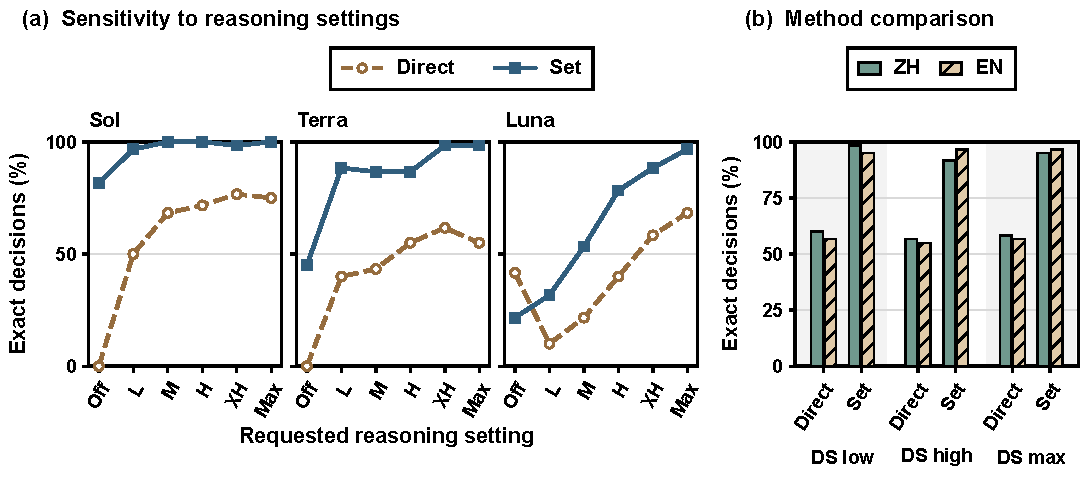
\includegraphics[width=\textwidth]{15_configuration_robustness.pdf}
\caption{\textbf{Method performance across reasoning settings and task languages.} (a) Sol, Terra, and Luna: 18 settings, 60 tasks per method. Off denotes none; L/M/H/XH denote low/medium/high/xhigh. (b) DeepSeek: 60 tasks per language and method. Plain bars denote Chinese (ZH), hatched bars English (EN). Tables~\ref{tab:grid} and~\ref{tab:language} give counts.}
\label{fig:robustness}
\end{figure*}

\begin{table*}[t]
\centering\small\setlength{\tabcolsep}{5pt}
\begin{tabular}{@{}llrrrr@{}}
\toprule
&&\multicolumn{2}{c}{Direct}&\multicolumn{2}{c}{SET}\\
Model & Setting & Exact/$n$ & U/R/O & Exact/$n$ & U/R/O\\
\midrule
Sol & off & 0/60 & 60/0/0 & 49/60 & 8/1/2\\
 & low & 30/60 & 9/20/1 & 58/60 & 2/0/0\\
 & medium & 41/60 & 3/16/0 & 60/60 & 0/0/0\\
 & high & 43/60 & 0/17/0 & 60/60 & 0/0/0\\
 & xhigh & 46/60 & 0/14/0 & 59/60 & 0/0/1\\
 & max & 45/60 & 0/15/0 & 60/60 & 0/0/0\\
\midrule
Terra & off & 0/60 & 59/0/1 & 27/60 & 8/3/22\\
 & low & 24/60 & 17/19/0 & 53/60 & 6/0/1\\
 & medium & 26/60 & 15/19/0 & 52/60 & 6/0/2\\
 & high & 33/60 & 7/20/0 & 52/60 & 5/0/3\\
 & xhigh & 37/60 & 8/14/1 & 59/60 & 1/0/0\\
 & max & 33/60 & 3/15/9 & 59/60 & 0/0/1\\
\midrule
Luna & off & 25/60 & 6/28/1 & 13/60 & 24/12/11\\
 & low & 6/60 & 44/10/0 & 19/60 & 28/6/7\\
 & medium & 13/60 & 40/7/0 & 32/60 & 20/2/6\\
 & high & 24/60 & 28/8/0 & 47/60 & 10/0/3\\
 & xhigh & 35/60 & 11/13/1 & 53/60 & 3/0/4\\
 & max & 41/60 & 4/12/3 & 58/60 & 2/0/0\\
\bottomrule
\end{tabular}
\caption{All complete GPT-5.6 reasoning settings: exact/$n$ and unsafe/false-refusal/other (U/R/O), with $n=60$ in every cell. The 18 configurations cover six settings each for Sol, Terra, and Luna. Settings denote requested effort, not equal or measured compute.}
\label{tab:grid}
\end{table*}

\subsection{Task Language}
\label{app:language}
We report paired Direct and SET evaluations on the same 60 task identifiers in Chinese and English. A reviewed 183-phrase translation map preserves quantities, types, events, and authorization, with system instructions held fixed. Table~\ref{tab:language} reports the complete Direct/SET outcomes for these paired 60-task runs. Across six DeepSeek setting--language cells, Direct achieves 33--36/60 exact decisions and SET 55--59/60 (Figure~\ref{fig:robustness}b). The results concern these controlled Chinese/English renderings, not language invariance in general.

\begin{table*}[t]
\centering\small\setlength{\tabcolsep}{4pt}
\begin{tabular}{@{}llrrrr@{}}
\toprule
&&\multicolumn{2}{c}{Direct}&\multicolumn{2}{c}{SET}\\
Configuration & Language & Exact/$n$ & U/R/O & Exact/$n$ & U/R/O\\
\midrule
DS low & ZH & 36/60 & 9/14/1 & 59/60 & 0/0/1\\
 & EN & 34/60 & 6/15/5 & 57/60 & 0/0/3\\
\midrule
DS high & ZH & 34/60 & 10/14/2 & 55/60 & 0/0/5\\
 & EN & 33/60 & 8/16/3 & 58/60 & 0/0/2\\
\midrule
DS max & ZH & 35/60 & 11/13/1 & 57/60 & 2/0/1\\
 & EN & 34/60 & 12/11/3 & 58/60 & 0/0/2\\
\midrule
Astra max & ZH & 55/60 & 0/4/1 & 60/60 & 0/0/0\\
 & EN & 49/60 & 0/9/2 & 60/60 & 0/0/0\\
\bottomrule
\end{tabular}
\caption{Language outcomes and failure partitions: ZH is Chinese and EN is English. U/R/O denotes unsafe/false-refusal/other. Each setting--language cell has $n=60$ per method. Figure~\ref{fig:robustness}b shows the DeepSeek subset.}
\label{tab:language}
\end{table*}

\subsection{Output-Budget Control}
\label{app:budget}
On 46 historically budget-sensitive Direct tasks, 92 new calls compare the original cap with 262,144 tokens under the same 1,800-second deadline. Exact decisions rise from 10/46 to 26/46, with unsafe acceptance and false refusal still observed. The original outcomes remain in their cohorts. Results on this selected subset do not estimate general failure rates.

\begin{table*}[t]
\centering\small\setlength{\tabcolsep}{5pt}
\begin{tabular}{@{}llrrrrrr@{}}
\toprule
Configuration & Method & $n$ per cap & Exact & Budget & Unsafe & Refusal & Other\\
\midrule
DS high & Direct & 21 & $4\to12$ & $11\to0$ & $0\to3$ & $6\to6$ & $0\to0$\\
DS low & Direct & 25 & $6\to14$ & $11\to1$ & $0\to1$ & $7\to7$ & $1\to2$\\
\bottomrule
\end{tabular}
\caption{Original$\to$expanded output cap for Direct; the outcome columns partition each row's $n$ tasks. Budget counts output-token exhaustion; Other denotes remaining value errors. Selection of historically budget-sensitive tasks limits prevalence estimates.}
\label{tab:budget}
\end{table*}
\section{Availability Study and Verification}
\label{app:permissionaudit}
\subsection{Design and frozen interventions}
\label{app:availability}
\paragraph{Tasks and frozen specifications.}
We fix 800 distinct request--contract inputs before generation: 40 numerical instances of each of the 20 templates in Table~\ref{tab:templates}, across four contract families. Each has 128 candidates. DeepSeek Flash (\texttt{deepseek-flash}), GLM (\texttt{glm-5.3}), and Qwen Max (\texttt{qwen3.8-max}) use low effort and a 32,768-token output budget. Preparation receives the request, contract, and schema, excluding candidates and reference information.

Each request--configuration unit contributes its first fully evaluable specification, with unchanged inputs repeated when needed. Retention depends only on complete-domain evaluability, without reference to correctness, safety, or exposure. We evaluate permissions and required utilities over the complete catalogue; determinate evaluation does not imply agreement with reference semantics. Percentages use all 800 planned units per model, or 2,400 overall. Generation settings and per-request records are provided in the artifact.

\paragraph{Catalogue construction and reference checks.}
The construction allocates 32 offers each to authorized positive-value purchases, unauthorized boundary cases, contract-branch controls, and ordinary sampled attributes. Construction categories differ from authorization labels: the latter two blocks may add authorized purchases. Boundary distances include one monetary subunit and approximately 1\%, 5\%, and 20\% of the risk limit. Attributes remain contract-consistent.

Each template has 20 S and 20 T requests. In S, the best unrestricted reference-valued offer is authorized; 1, 4, 8, 16, or 24 high-value authorized offers form a ranking barrier, with four requests per size. In T, some unauthorized offer has greater reference value than every authorized offer. These strata and all candidates are fixed before generation. The study therefore probes a controlled pressure distribution. Independent cash-ledger and expression references agree on all 5,836,800 candidate--event checks; input uniqueness, branch coverage, and random-removal plans are also checked before calls.

S provides opportunities for a false admission to be masked by an authorized reference-valued winner; T makes unauthorized alternatives more attractive under the reference. Neither stratum fixes the generated permissions. Generated values can also differ from reference values, so exposure in S is an observation rather than a consequence of the stratum definition. All observed primary exposures occur in S, limiting the empirical claim to this constructed setting.

\paragraph{Frozen interventions and endpoint.}
The original catalogue, 128 random-removal conditions (32 each for $k\in\{1,4,8,16\}$), 16 generated-rank prefixes, and one unauthorized-only catalogue define 146 conditions per specification. Random plans are fixed in advance and shared across models. Ranked removals order originally admitted offers by generated utility, retaining original candidate order for ties; the removal rule uses no reference labels. Surviving attributes, permissions, utilities, and the selector remain unchanged. The unauthorized-only condition retains all reference-unauthorized offers and is an extreme control.

The primary endpoint requires an originally safe acceptance, an unauthorized selection for some prefix of at most eight removals, and at least one surviving offer permitted and positively valued under both generated conditions and the reference. Each specification counts once per budget. Refusals do not count as safe purchases. Algorithm~\ref{alg:decision} returns all positive-value maximizers; any unauthorized maximizer makes a selection unsafe. Mixed-authorization ties and fixed-first selection are checked separately. Cumulative exposure is distinct from the outcome at exactly $k$ removals, which may return to safety after an unauthorized winner is itself removed.

\subsection{Complete results and controls}
\label{app:availability-results}
The retained cohort contains 2,373 fully evaluable specifications, including 2,298 initially safe purchases and 2,221 exact purchases. The primary endpoint occurs in 48 of the former (2.09\%) and eight of the latter (0.36\%). Ten exact purchases have false admissions (0.45\%), of which eight are exposed within the primary budget. Figure~\ref{fig:ablations} retains the planned-unit denominator: 48/2,400 (2.00\%). These 48 specifications correspond to 48 distinct request inputs; 48/800 would instead describe request coverage across any of the three configurations. Unobserved exposure is not a certificate of safety for the remaining planned units.

\begin{table}[!t]
\centering\small\setlength{\tabcolsep}{3pt}
\begin{tabular}{@{}lrrrr@{}}
\toprule
Model & Hidden (\%) & Exposed (\%) & Requests & Templates\\
\midrule
DeepSeek & 1.50 & 1.50 & 12 & 3\\
GLM & 6.88 & 4.13 & 33 & 12\\
Qwen & 0.50 & 0.38 & 3 & 3\\
\midrule
All & 2.96 & 2.00 & 48 & 15\\
\bottomrule
\end{tabular}
\caption{Availability outcomes over the planned cohort. Hidden counts safe purchases concealing false admissions; Exposed requires a transition within eight removals with a viable authorized alternative. Requests and Templates count exposure coverage.}
\label{tab:availability-models}
\end{table}

\begin{table}[t]
\centering\small\setlength{\tabcolsep}{3pt}
\begin{tabular}{@{}lrrr@{}}
\toprule
Template & Hidden (\%) & Exposed (\%) & Requests\\
\midrule
a1 & 4.17 & 1.67 & 2\\
a2 & 0.00 & 0.00 & 0\\
a3 & 5.00 & 2.50 & 3\\
a4 & 1.67 & 1.67 & 2\\
a5 & 9.17 & 5.83 & 7\\
\midrule
b1 & 1.67 & 1.67 & 2\\
b2 & 0.00 & 0.00 & 0\\
b3 & 0.00 & 0.00 & 0\\
b4 & 0.83 & 0.83 & 1\\
b5 & 3.33 & 1.67 & 2\\
\midrule
c1 & 1.67 & 0.83 & 1\\
c2 & 5.00 & 4.17 & 5\\
c3 & 0.00 & 0.00 & 0\\
c4 & 0.83 & 0.83 & 1\\
c5 & 6.67 & 2.50 & 3\\
\midrule
d1 & 3.33 & 3.33 & 4\\
d2 & 2.50 & 2.50 & 3\\
d3 & 5.83 & 5.00 & 6\\
d4 & 0.83 & 0.00 & 0\\
d5 & 6.67 & 5.00 & 6\\
\bottomrule
\end{tabular}
\caption{All 20 templates, including zero-event structures. Percentages use each template's planned cohort across models. Shared requests and numerical variants are not independent logical structures.}
\label{tab:availability-templates}
\end{table}

\paragraph{Coverage, controls, and verification.}
The primary endpoint covers \AvailExposedRequests{} distinct requests, \AvailExposedTemplates{} templates, four families, and three configurations. All its witnesses occur in the predeclared S stratum; the family counts are 14 coupon, five insurance, ten return, and nineteen replacement cases. Coverage is uneven: DeepSeek's cases remain concentrated in service replacement. The endpoint holds with wholly unauthorized maximizing sets in every case, so no primary witness relies on a mixed-authorization tie. The minimum witnesses retain \AvailBackupMin{}--\AvailBackupMax{} viable authorized alternatives. Eight exposed outputs began with exact decisions, covering four templates and two model configurations.

Every observed transition and attainable minimum-deletion witness is independently selected from the candidate matrix and replayed through the original expressions. Native permissions and values must equal the corresponding subset of the original matrix. Certificates retain the violating reference loss, selected maximizing set, surviving alternatives, and source hashes. These checks validate the controlled mechanism; they do not estimate deployment frequency.

\begin{table}[!t]
\centering\small\setlength{\tabcolsep}{3pt}
\begin{tabular}{@{}lrrrr@{}}
\toprule
Budget $k$ & 1 & 4 & 8 & 16\\
\midrule
Directed safe to unsafe & 0.71 & 1.42 & 2.00 & 2.54\\
Directed unsafe to safe & 0.29 & 0.79 & 1.21 & 1.54\\
Random safe to unsafe & 0.001 & 0.034 & 0.035 & 0.103\\
Random unsafe to safe & 0.003 & 0.009 & 0.014 & 0.044\\
\bottomrule
\end{tabular}
\caption{Availability controls as percentages of all planned trials. Directed rows count whether a transition occurs at any prefix within the budget; random rows average observed transition fractions over 32 draws per trial. Safe-to-unsafe requires a viable authorized alternative. Forward and reverse cumulative events need not occur at the same prefix.}
\label{tab:availability-controls}
\end{table}

Across all 71 initially safe specifications with false admissions, the unauthorized-only control exposes a positive-valued unauthorized offer. Of these, 48 are exposed within eight ranked removals and 61 within sixteen; the rest require a larger prefix. Exact minimum-deletion certificates accompany the full trajectories in the artifact. Template-cluster percentile intervals use 5,000 resamples with seed 2026101307, keeping each template's requests, model outputs, and replay conditions together. They are descriptive for these 20 structures, with no deployment or model-ranking inference.

Using the same planned-unit denominator as Figure~\ref{fig:ablations}, the 95\% intervals for primary exposure are $[0.00,3.50]\%$ for DeepSeek, $[2.13,6.38]\%$ for GLM, and $[0.00,0.75]\%$ for Qwen. The corresponding hidden-error intervals are $[0.00,3.50]\%$, $[3.75,10.38]\%$, and $[0.00,1.13]\%$. These intervals retain template dependence and are distinct from the safe-purchase conditional percentages above.

\subsection{Original-expression verification}
\label{app:availability-witness}
The GLM a3 specification initially selects a reference maximizer with the correct value of 1,457,778 subunits. It contains one state record whose risk expression includes all 57 event terms. For event $\{0,1,3,5\}$, two partial-cancellation group charges must be added before the group cap: the correct capped charge is 19,500, but the expression includes only the second charge, yielding 9,900. Event coverage alone therefore does not ensure correct contractual aggregation.

After four originally higher-ranked offers become unavailable, the admitted unauthorized offer wins with generated value 1,359,878, ahead of the best surviving authorized value 1,257,378. Its true worst loss is 268,094 against a 267,994 limit; the specification's maximum is 263,194. The difference in this event's omitted charge is 9,600, whereas the difference between the two worst losses is 4,900; the maxima arise from different event calculations. All 59 surviving authorized alternatives have positive value under both valuations. The request, conditions, remaining attributes, and selector are unchanged. Original expressions, event ledgers, and the complete candidate-level certificate are provided in the artifact.


\paragraph{Archived exploratory scope.}
The artifact separately archives earlier catalogue probes, selected-output component interventions, supplied-reading tests, and exploratory input, price, and component changes. They use different cohorts and are not pooled with this study. Selected reversals were accompanied by non-triggering checks and improving transitions; they do not establish that more accurate valuation generally increases unsafe purchasing. Complete protocols and positive and negative outcomes remain in the archival reports.
\end{document}
